% **************************************************************************************************************
% A Classic Thesis Style
% An Homage to The Elements of Typographic Style
%
% Copyright (C) 2009 André Miede http://www.miede.de
%
% If you like the style then I would appreciate a postcard. My address 
% can be found in the file ClassicThesis.pdf. A collection of the 
% postcards I received so far is available online at 
% http://postcards.miede.de
%
% License:
% This program is free software; you can redistribute it and/or modify
% it under the terms of the GNU General Public License as published by
% the Free Software Foundation; either version 2 of the License, or
% (at your option) any later version.
%
% This program is distributed in the hope that it will be useful,
% but WITHOUT ANY WARRANTY; without even the implied warranty of
% MERCHANTABILITY or FITNESS FOR A PARTICULAR PURPOSE.  See the
% GNU General Public License for more details.
%
% You should have received a copy of the GNU General Public License
% along with this program; see the file COPYING.  If not, write to
% the Free Software Foundation, Inc., 59 Temple Place - Suite 330,
% Boston, MA 02111-1307, USA.
%
% **************************************************************************************************************
% Note:
%    * You must not use "u etc. in strings/commands that will be spaced out (use \"u or real umlauts instead)
%    * Chapters must be marked with the \myChapter{Foo} command (sorry for the inconvenience at this point)
%    * New enumeration (small caps): \begin{aenumerate} \end{aenumerate}
%    * For margin notes: \graffito{}
%    * Do not use bold fonts in this style, it is designed around them
%    * Use tables as in the examples
%    * See classicthesis-ldpkg.sty for useful commands
% **************************************************************************************************************
% To Do:
%    * fix space at beginning of List of Listings 
%    * mathbb in section-titles/chapter-titles => disappears somehow in headlines!!!
%    * think about processing a4paper, a5paper, 10pt, 11pt, 12pt etc. options for typearea layout
%      (store values in internal variables and handle by \AtEndOfPackage{\areaset...})
% **************************************************************************************************************
\documentclass[ twoside,openright,titlepage,fleqn,pointlessnumbers,headinclude,%1headlines,% 
                10pt,a4paper,BCOR5mm,footinclude,cleardoubleempty,abstractoff % <--- obsolete, remove (todo)
                ]{scrreprt}

\usepackage[utf8]{inputenc}
\usepackage[OT4]{polski}


\usepackage{moreverb}
\let\verbatiminput=\verbatimtabinput
\def\verbatimtabsize{4\relax}

%\usepackage{listings}
\usepackage{algorithm}
\usepackage{algorithmic}
\floatname{algorithm}{Algorytm}
\renewcommand{\listalgorithmname}{Spis algorytmów}
\renewcommand{\algorithmicrequire}{\textbf{Asercje początkowe:}}
% ********************************************************************
% KOMA-Script setup http://www.komascript.de/betaKOMAoptions
% ********************************************************************
%\KOMAoptions{%
%    paper=a4,%
%    fontsize=10pt,%
%    cleardoublepage=empty%
%    %,footinclude=true%
%    %,abstract=false%
%}
% ********************************************************************
% Development Stuff
% ********************************************************************
\listfiles
%\usepackage[l2tabu, orthodox, abort]{nag}
%\usepackage[warning, all]{onlyamsmath}
% ********************************************************************
% Re-usable information
% ********************************************************************
\newcommand{\myTitle}{System śledzenia ruchów 6DOF\xspace}
\newcommand{\myDegree}{System śledzący ruchy użytkownika w sześciu stopniach swobody\xspace}
\newcommand{\myName}{Michał Janiszewski\xspace}
\newcommand{\myProf}{dr inż. Adam Wojciechowski\xspace}
\newcommand{\myOtherProf}{Put name here\xspace}
\newcommand{\mySupervisor}{Put name here\xspace}
\newcommand{\myFaculty}{Wydział Fizyki Technicznej, Informatyki i Matematyki Stosowanej\xspace}
\newcommand{\myDepartment}{Put data here\xspace}
\newcommand{\myUni}{\protect{Politechnika Łódzka}\xspace}
\newcommand{\myLocation}{Zgierz\xspace}
\newcommand{\myTime}{Grudzień 2010\xspace}
\newcommand{\myVersion}{Wersja 0.1\xspace}
%*******************************************************
% Packages with options that might require adjustments
%*******************************************************
\usepackage[english,polish]{babel}           
\usepackage[square,numbers]{natbib}

\usepackage{multicol}

\let\orgtheindex\theindex
\let\orgendtheindex\endtheindex
\def\theindex{%
\def\twocolumn{\begin{multicols}{2}}%
\def\onecolumn{}%
\clearpage
\orgtheindex
}
\def\endtheindex{%
\end{multicols}%
\orgendtheindex
}


\usepackage{makeidx}
\makeindex
% save and then undefine the conflicting command
% we need \makeatletter because \@undefined uses the special @ character.
\makeatletter
\let\amslll\lll
\let\lll\@undefined
\makeatother

\usepackage{amssymb}
\usepackage[fleqn]{amsmath} % math environments and more by the AMS

% taken form minted, distributed under LaTeX Project Public License 1.3 or later (http://www.latex-project.org/lppl.txt): http://code.google.com/p/minted/
\newfloat{listing}{h}{lol2}
\newcommand\listingscaption{Listing}
\floatname{listing}{\listingscaption}
\newcommand\listoflistingscaption{Spis listingów}
\providecommand\listoflistings{\listof{listing}{\listoflistingscaption}}

%*******************************************************
\usepackage{classicthesis-ldpkg}
%*******************************************************
% Options for classicthesis.sty:
% tocaligned eulerchapternumbers drafting linedheaders listsseparated 
% subfig nochapters beramono eulermath parts minionpro pdfspacing 
% listings dottedtoc
\usepackage[eulerchapternumbers,pdfspacing,
            subfig,beramono,eulermath,dottedtoc]{classicthesis}
\renewcommand{\lstlistlistingname}{\listoflistingscaption}
%*******************************************************            
%\usepackage[section,below]{placeins} <--- not everybody wants this
%\usepackage[all]{hypcap} <--- does not work with MiKTeX 2.6
% ********************************************************************
% Language/strings for backrefs (change here, thanks, Lorenzo)
%*******************************************************
%\renewcommand{\backrefnotcitedstring}{\relax}%(Not cited.)
%\renewcommand{\backrefcitedsinglestring}[1]{(Citato a pagina~#1.)}
%\renewcommand{\backrefcitedmultistring}[1]{(Citato alle pagine~#1.)}
%\renewcommand{\backreftwosep}{ e~}
%\renewcommand{\backreflastsep}{ e~}
% ********************************************************************
% Setup and Finetuning
%*******************************************************
\newlength{\abcd} % for ab..z string length calculation
\newcommand{\myfloatalign}{\centering} % how all the floats will be aligned
\setlength{\extrarowheight}{3pt} % increase table row height
% ********************************************************************
% Captions look and feel
%*******************************************************
\captionsetup{format=hang,font=small}
% ********************************************************************
% Listings setup
% ********************************************************************
%\lstset{emph={trueIndex,root},emphstyle=\color{BlueViolet}}%\underbar} % for special keywords
% ********************************************************************
\lstset{language=[LaTeX]Tex,%C++,
    keywordstyle=\color{RoyalBlue},%\bfseries,
    basicstyle=\small\ttfamily,
    %identifierstyle=\color{NavyBlue},
    commentstyle=\color{Green}\ttfamily,
    stringstyle=\rmfamily,
    numbers=none,%left,%
    numberstyle=\scriptsize,%\tiny
    stepnumber=5,
    numbersep=8pt,
    showstringspaces=false,
    breaklines=true,
    tabsize=4,
    %frame=L
} 
% ********************************************************************
% Where to look for graphics
%*******************************************************
%\graphicspath{{gfx/}{misc/}} % considered harmful according to l2tabu
% ********************************************************************
% Hyperreferences
%*******************************************************
\hypersetup{%
    colorlinks=true, linktocpage=true, pdfstartpage=3, pdfstartview=FitV,%
    % uncomment the following line if you want to have black links (e.g., for printing)
    %colorlinks=false, linktocpage=false, pdfborder={0 0 0}, pdfstartpage=3, pdfstartview=FitV,% 
    breaklinks=true, pdfpagemode=UseNone, pageanchor=true, pdfpagemode=UseOutlines,%
    plainpages=false, bookmarksnumbered, bookmarksopen=true, bookmarksopenlevel=1,%
    hypertexnames=true, pdfhighlight=/O,%hyperfootnotes=true,%nesting=true,%frenchlinks,%
    urlcolor=webbrown, linkcolor=RoyalBlue, citecolor=webgreen, %pagecolor=RoyalBlue,%
    %urlcolor=Black, linkcolor=Black, citecolor=Black, %pagecolor=Black,%
    pdftitle={\myTitle},%
    pdfauthor={\textcopyright\ \myName, \myUni, \myFaculty},%
    pdfsubject={},%
    pdfkeywords={},%
    pdfcreator={pdfLaTeX},%
    pdfproducer={LaTeX with hyperref and classicthesis}%
}


\usepackage{rotating}
\usepackage{pdfpages}
%********************************************************************
% Hyphenation
%*******************************************************
%\hyphenation{put special hyphenation here}
% ********************************************************************
% GO!GO!GO! MOVE IT!
%*******************************************************
\begin{document}
%********************************************************************
% Frontmatter
%*******************************************************
\frenchspacing
\raggedbottom
\selectlanguage{polish} % american ngerman
%\renewcommand*{\bibname}{new name}
%\setbibpreamble{}
\pagenumbering{roman}
\pagestyle{plain}
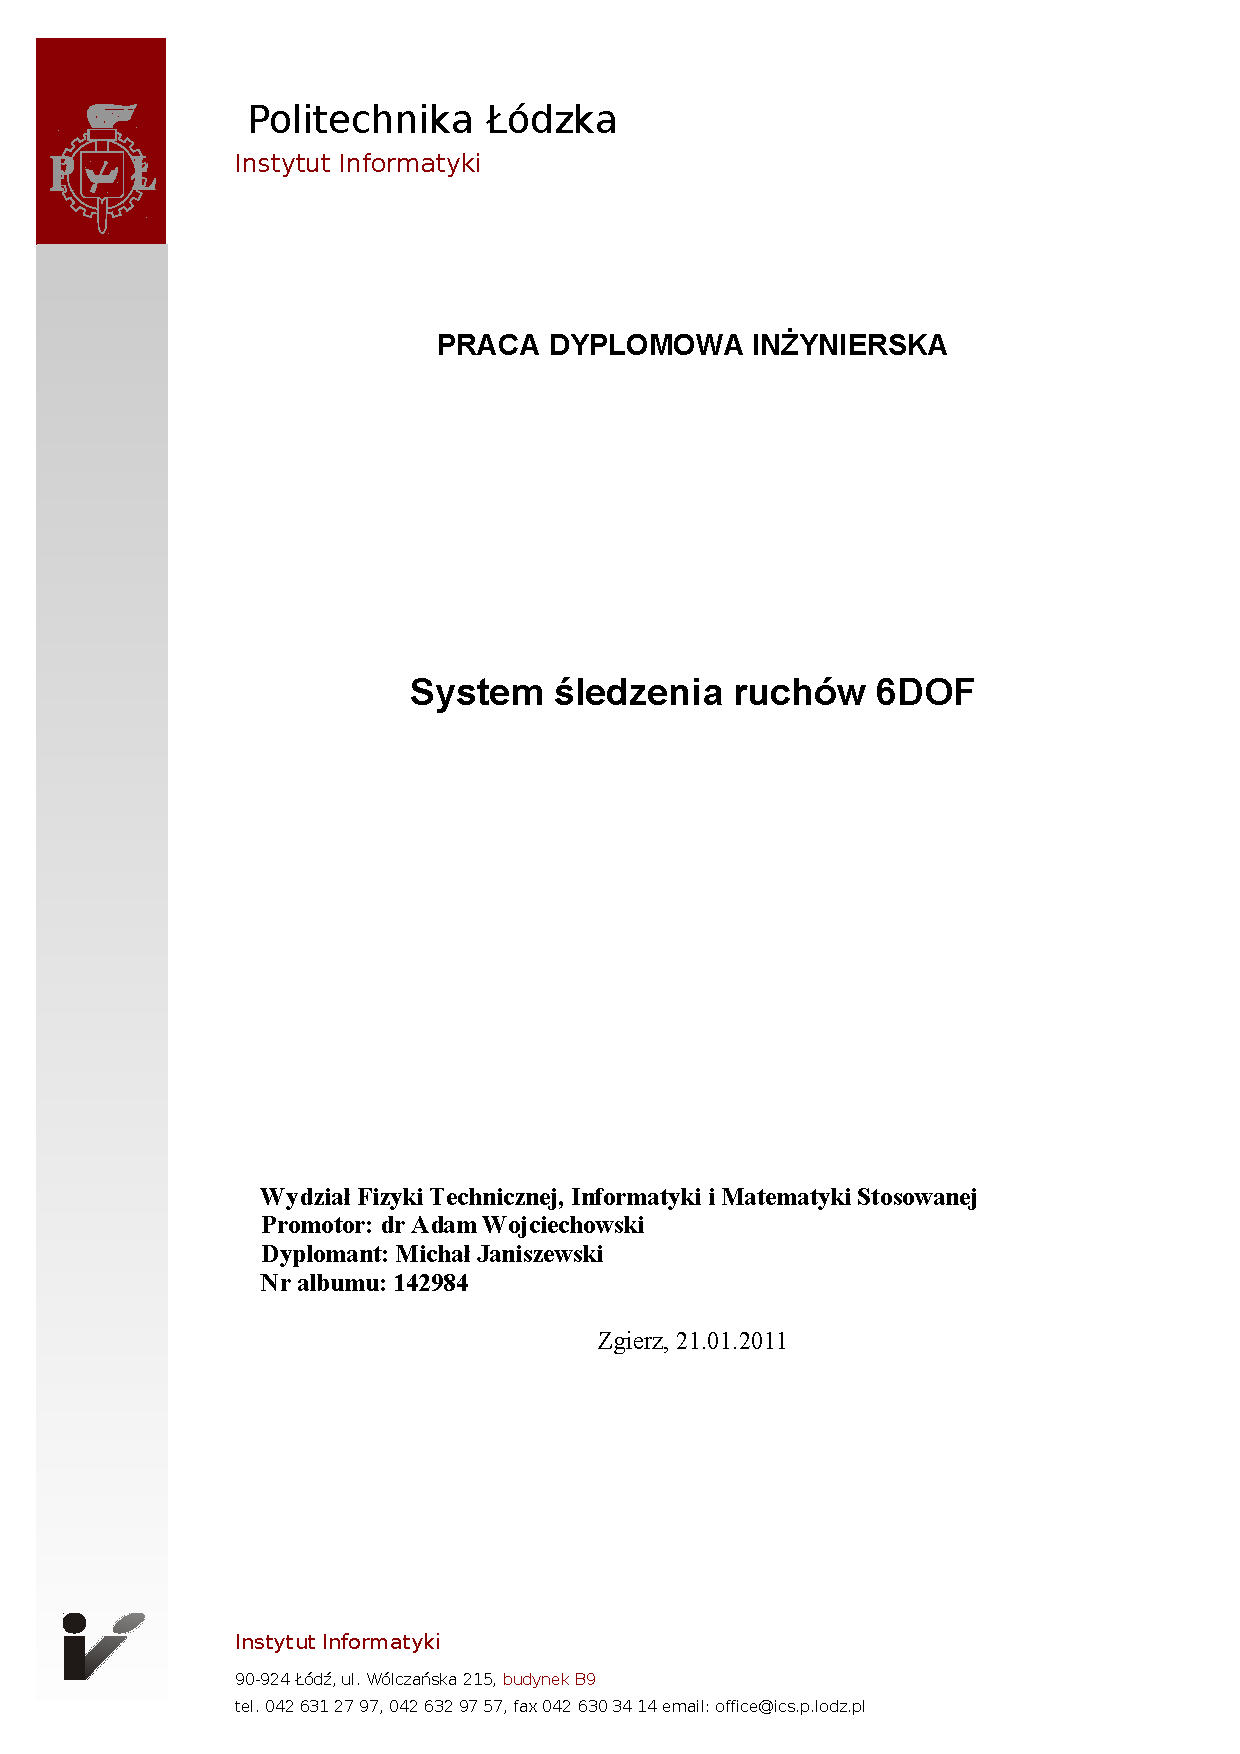
\includepdf[pagecommand={\thispagestyle{empty}}]{FrontBackmatter/front_pl.pdf}
%*******************************************************
% Titlepage
%*******************************************************
\begin{titlepage}
	% if you want the titlepage to be centered, uncomment and fine-tune the line below (KOMA classes environment)
	\begin{addmargin}[-1cm]{-3cm}
    \begin{center}
        \large  

        \hfill

        \vfill

        \begingroup
            \color{Maroon}\spacedallcaps{\myTitle} \\ \bigskip
        \endgroup

        \spacedlowsmallcaps{\myName}

        \vfill

        \includegraphics[width=6cm]{gfx/TFZsuperellipse_bw} \\ \medskip

        \myDegree \\ \medskip   
        %\myDepartment \\                            
        %\myFaculty \\
        %\myUni \\ \bigskip

        \myTime

        \vfill                      

    \end{center}  
  \end{addmargin}       
\end{titlepage}   
\thispagestyle{empty}

\hfill

\vfill

\noindent\myName: \textit{\myTitle,} \myDegree, \textcopyright\ \myTime

%\bigskip
%
%\noindent\spacedlowsmallcaps{Supervisors}: \\
%\myProf \\
%\myOtherProf \\ 
%\mySupervisor
%
%\medskip
%
%\noindent\spacedlowsmallcaps{Location}: \\
%\myLocation
%
%\medskip
%
%\noindent\spacedlowsmallcaps{Time Frame}: \\
%\myTime

%\cleardoublepage%*******************************************************
% Dedication
%*******************************************************
\thispagestyle{empty}
%\phantomsection 
\refstepcounter{dummy}
\pdfbookmark[1]{Dedication}{Dedication}

\vspace*{3cm}

\begin{center}
    \emph{Ohana} means family. \\
    Family means nobody gets left behind, or forgotten. \\ \medskip
    --- Lilo \& Stitch    
\end{center}

\medskip

\begin{center}
    Dedicated to the loving memory of Rudolf Miede. \\ \smallskip
    1939\,--\,2005
\end{center}
%\cleardoublepage%*******************************************************
% Abstract
%*******************************************************
%\renewcommand{\abstractname}{Abstract}
\pdfbookmark[1]{Abstract}{Abstract}
\begingroup
\let\clearpage\relax
\let\cleardoublepage\relax
\let\cleardoublepage\relax

\chapter*{Abstract}
Short summary of the contents in English\dots


\vfill

\pdfbookmark[1]{Zusammenfassung}{Zusammenfassung}
\chapter*{Zusammenfassung}
Kurze Zusammenfassung des Inhaltes in deutscher Sprache\dots


\endgroup			

\vfill
%\cleardoublepage%*******************************************************
% Publications
%*******************************************************
\pdfbookmark[1]{Publications}{publications}
\chapter*{Publications}
Some ideas and figures have appeared previously in the following publications:

\bigskip

\noindent Put your publications from the thesis here.
%\cleardoublepage%*******************************************************
% Acknowledgments
%*******************************************************
\pdfbookmark[1]{Acknowledgments}{acknowledgments}

\begin{flushright}{\slshape    
    We have seen that computer programming is an art, \\ 
    because it applies accumulated knowledge to the world, \\ 
    because it requires skill and ingenuity, and especially \\
    because it produces objects of beauty.} \\ \medskip
    --- \defcitealias{knuth:1974}{Donald E. Knuth}\citetalias{knuth:1974} \citep{knuth:1974}
\end{flushright}



\bigskip

\begingroup
\let\clearpage\relax
\let\cleardoublepage\relax
\let\cleardoublepage\relax
\chapter*{Acknowledgments}
Put your acknowledgments here.

Many thanks to everybody who already sent me a postcard!

Regarding the typography and other help, many thanks go to Marco 
Kuhlmann, Philipp Lehman, Lothar Schlesier, Jim Young, Lorenzo 
Pantieri and Enrico Gregorio\footnote{Members of GuIT (Gruppo 
Italiano Utilizzatori di \TeX\ e \LaTeX )}, J\"org Sommer, 
Joachim K\"ostler, Daniel Gottschlag, Denis Aydin, Paride 
Legovini, Steffen Prochnow, Nicolas Repp, 
and the whole \LaTeX-community for support, ideas and some great software.

\endgroup




\pagestyle{scrheadings}
\cleardoublepage%*******************************************************
% Table of Contents
%*******************************************************
%\phantomsection
\refstepcounter{dummy}
\pdfbookmark[1]{\contentsname}{tableofcontents}
\setcounter{tocdepth}{2} % <-- 2 includes up to subsections in the ToC
\setcounter{secnumdepth}{3} % <-- 3 numbers up to subsubsections
\manualmark
\markboth{\spacedlowsmallcaps{\contentsname}}{\spacedlowsmallcaps{\contentsname}}
\tableofcontents 
\automark[section]{chapter}
\renewcommand{\chaptermark}[1]{\markboth{\spacedlowsmallcaps{#1}}{\spacedlowsmallcaps{#1}}}
\renewcommand{\sectionmark}[1]{\markright{\thesection\enspace\spacedlowsmallcaps{#1}}}%*******************************************************
% List of Figures and of the Tables
%*******************************************************
\clearpage

\begingroup 
    \let\clearpage\relax
    \let\cleardoublepage\relax
    \let\cleardoublepage\relax
    %*******************************************************
    % List of Figures
    %*******************************************************    
    %\phantomsection 
    \refstepcounter{dummy}
    %\addcontentsline{toc}{chapter}{\listfigurename}
    \pdfbookmark[1]{\listfigurename}{lof}
    \listoffigures

    \vspace*{8ex}

    %*******************************************************
    % List of Tables
    %*******************************************************
    %\phantomsection 
    \refstepcounter{dummy}
    %\addcontentsline{toc}{chapter}{\listtablename}
    \pdfbookmark[1]{\listtablename}{lot}
    \listoftables
        
    \vspace*{8ex}
%   \newpage
    
    %*******************************************************
    % List of Listings
    %*******************************************************      
	  %\phantomsection 
    \refstepcounter{dummy}
    %\addcontentsline{toc}{chapter}{\lstlistlistingname}
    \pdfbookmark[1]{\lstlistlistingname}{lol2}
    \listoflistings
    \vspace*{8ex}

    %*******************************************************
    % List of Algorithms
    %*******************************************************      
	  %\phantomsection 
    \refstepcounter{dummy}
    %\addcontentsline{toc}{chapter}{\lstlistlistingname}
    \pdfbookmark[1]{\listalgorithmname}{loa}
    \listofalgorithms
    \vspace*{8ex}

    \vspace*{8ex}
       
    %*******************************************************
    % Acronyms
    %*******************************************************
    %\phantomsection 
    \refstepcounter{dummy}
    \pdfbookmark[1]{Indeks}{indeks}
    \markboth{\spacedlowsmallcaps{Indeks}}{\spacedlowsmallcaps{Indeks}}
    \printindex
\endgroup

\cleardoublepage
%********************************************************************
% Mainmatter
%*******************************************************
\pagenumbering{arabic}
% use \cleardoublepage here to avoid problems with pdfbookmark
%\cleardoublepage\myPart{Wstęp}
%************************************************
\myChapter{Wstęp}\label{ch:wstep}
%************************************************

Systemy śledzenia ruchów to pojęcie, które obejmuje szeroką gamę zestawów składających się z urządzeń dostarczających danych o położeniu oraz wyspecjalizowanego oprogramowania, które te informacje przetwarza. Systemy takie, w ogólnym ujęciu, można spotkać w wielu miejscach:
\begin{aenumerate}
  \item w fabrykach śledzone jest przemieszczanie się produktów w celu ich dystrybucji,
  \item zarówno w produkcji gier jak i filmów stosuje się systemy \textsl{motion capture}, czyli przechwytywania ruchów,
  \item systemem śledzenia ruchów można nazwać także fotoradar przy drodze,
  \item cyfrowe modelowanie, w celu odtworzenia wirtualnego modelu istniejącego przedmiotu, często posługuje się systemem śledzenia ruchów pod postacią digitizera.
\end{aenumerate}

W każdym przypadku zarówno metoda pozyskiwania danych, protokół, którym są przekazywane oraz oprogramowanie te dane odbierające i przetwarzające jest inne, gdyż inne są wymagania, założenia i konstrukcja każdego z tych systemów.

Spośród mnogiej ilości zastosowań takich systemów najbardziej interesującym z mojego punktu widzenia jest śledzenie ruchów na potrzeby odwzorowania ich w grach wideo.

W swojej pracy przybliżę istniejące systemy wykorzystywane w konsolach w dniu dzisiejszym oraz zaprezentuję metodę śledzenia ruchów, jaka nie została dotychczas wykorzystana na potrzeby gier wideo.


% 
% This bundle for \LaTeX\ has two goals:
% \begin{enumerate}
%     \item Provide students with an easy-to-use template for their
%     Master's
%     or PhD thesis. (Though it might also be used by other types of
%     authors
%     for reports, books, etc.)
%     \item Provide a classic, high quality typographic style which is
%     inspired by \cauthor{bringhurst:2002}'s ``\emph{The Elements of
%     Typographic Style}'' \citep{bringhurst:2002}.
%     \graffito{\myTitle \myVersion}
% \end{enumerate}
% The bundle is configured to run with a \emph{full} 
% MiK\TeX\ or \TeX Live\footnote{See the file \texttt{LISTOFFILES} for
% needed packages. Furthermore, \texttt{classicthesis} 
% works with most other distributions and, thus, with most operating 
% systems \LaTeX\ is available for.} 
% installation right away and, therefore, it uses only freely available 
% fonts. (Minion fans can easily adjust the style to their needs.)
% 
% People interested only in the nice style and not the whole bundle can
% now use the style stand-alone via the file \texttt{classicthesis.sty}.
% This works now also with ``plain'' \LaTeX.
% 
% This should enable anyone with a basic knowledge of \LaTeXe\ to
% produce beautiful documents without too much effort. In the end, this
% is my overall goal: more beautiful documents, especially theses, as I
% am tired of seeing so many ugly ones.
% 
% The whole template and the used style is released under the
% \textsmaller{GNU} General Public License. 
% 
% If you like the style then I would appreciate a postcard:
% \begin{center}
%  Andre Miede \\
%  Detmolder Strase 32 \\
%  31737 Rinteln \\
%  Germany
% \end{center}
% The postcards I got so far are available at \url{http://postcards.miede.de}.
% 
% Hopefully, this thesis template is done well enough for your needs and
% does not have too many flaws. So far, a couple of theses have been
% typeset successfully with it. If you are interested in some
% typographic details behind it, enjoy Robert Bringhurst's wonderful book.
% 
% \graffito{A well-balanced line width improves the legibility of
% the text. That's what typography is all about, right?}
% \paragraph{Important Note:} Some things of this style might look
% unusual at first glance, many people feel so in the beginning.
% However, all things are intentionally designed to be as they are,
% especially these:
% \begin{itemize}
%     \item No bold fonts are used. Italics or spaced small caps do the
%     job quite well.
%     \item The size of the text body is intentionally shaped like it
%     is. It supports both legibility and allows a reasonable amount of
%     information to be on a page. And, no: the lines are not too short.
%     \item The tables intentionally do not use vertical or double
%     rules. See the documentation for the \texttt{booktabs} package for
%     a nice discussion of this topic.\footnote{To be found online at \\
%     \url{http://www.ctan.org/tex-archive/macros/latex/contrib/booktabs/}.}
%     \item And last but not least, to provide the reader with a way
%     easier access to page numbers in the table of contents, the page
%     numbers are right behind the titles. Yes, they are \emph{not}
%     neatly aligned at the right side and they are \emph{not} connected
%     with dots that help the eye to bridge a distance that is not
%     necessary. If you are still not convinced: is your reader
%     interested in the page number or does she want to sum the numbers
%     up?
% \end{itemize}
% Therefore, please do not break the beauty of the style by changing
% these things unless you really know what you are doing! Please.
% 
% 
% \section{Organization}
% A very important factor for successful thesis writing is the
% organization of the material. This template suggests a structure as
% the following:
% \begin{itemize}
%     \graffito{You can use these margins for summaries of the text
%     body\dots}
%     \item\texttt{Chapters/} is where all the ``real'' content goes in
%     separate files such as \texttt{Chapter01.tex} etc.
%  %  \item\texttt{Examples/} is where you store all listings and other
%  %  examples you want to use for your text.
%     \item\texttt{FrontBackMatter/} is where all the stuff goes that
%     surrounds the ``real'' content, such as the acknowledgments,
%     dedication, etc.
%     \item\texttt{gfx/} is where you put all the graphics you use in
%     the thesis. Maybe they should be organized into subfolders
%     depending on the chapter they are used in, if you have a lot of
%     graphics.
%     \item\texttt{Bibliography.bib}: the Bib\TeX\ database to organize
%     all the references you might want to cite.
%     \item\texttt{classicthesis.sty}: the style definition to get this
%     awesome look and feel. 
%     \item\texttt{ClassicThesis.tcp} a \TeX nicCenter project file.
%     Great tool and it's free!
%     \item\texttt{ClassicThesis.tex}: the main file of your thesis
%     where all gets bundled together.
%     \item\texttt{classicthesis-ldpkg.sty}: a central place to load all 
%     nifty packages that are used. The package has only one option 
%     available, \texttt{nochapters}, which defaults to \texttt{false}.
%     Activate it if you want to use the package with a class which does
%     not have chapter divisions, \eg, an article.
% \end{itemize}
% This should get you started in no time.
% 
% 
% \section{Style Options}
% There are a couple of options for \texttt{classicthesis.sty} that
% allow for a bit of freedom concerning the layout:
% \begin{itemize}
%     \graffito{\dots or your supervisor might use the margins for some
%     comments of her own while reading.}
%     \item\texttt{drafting}: prints the date and time at the bottom of
%     each page, so you always know which version you are dealing with.
%     Might come in handy not to give your Prof. that old draft.
%     \item\texttt{eulerchapternumbers}: use figures from Hermann Zapf's
%     Euler math font for the chapter numbers. By default, old style
%     figures from the Palatino font are used.
%     \item\texttt{linedheaders}: changes the look of the chapter
%     headings a bit by adding a horizontal line above the chapter
%     title. The chapter number will also be moved to the top of the
%     page, above the chapter title.
%     \item\texttt{listsseparated}: will add extra space between table
%     and figure entries of different chapters in the list of tables or
%     figures, respectively.
%     \item\texttt{tocaligned}: aligns the whole table of contents on
%     the left side. Some people like that, some don't.
%     \item\texttt{subfig}(\texttt{ure}): is passed to the \texttt{tocloft} 
%     package to enable compatibility with the \texttt{subfig}(\texttt{ure}) 
%     package.
%     \item\texttt{nochapters}: allows to use the look-and-feel with 
%     classes that do not use chapters, \eg, for articles. Automatically
%     turns off a couple of other options: \texttt{eulerchapternumbers}, 
%     \texttt{linedheaders}, \texttt{listsseparated}, and \texttt{parts}.
%     \item\texttt{beramono}: loads Bera Mono as typewriter font. 
%     (Default setting is using the standard CM typewriter font.)
%     \item\texttt{eulermath}: loads the awesome Euler fonts for math. 
%     (Palatino is used as default font.)
%     \item\texttt{parts}: if you use Part divisions for your document,
%     you should choose this option. It provides you with the command
%     \verb|\myPart{}| which takes care of the style and the entry
%     into the Table of Contents. (Cannot be used together with
%     \texttt{nochapters}.)
%     \item\texttt{a5paper}: adjusts the page layout according to the
%     global \texttt{a5paper} option (\emph{experimental} feature).
%     \item\texttt{minionpro}: sets Robert Slimbach's Minion as the 
%     main font of the document. The textblock size is adjusted 
%     accordingly. 
%     \item\texttt{pdfspacing}: makes use of pdftex' letter spacing
%     capabilities via the \texttt{microtype} package.\footnote{Use 
%     \texttt{microtype}'s \texttt{DVIoutput} option to generate
%     DVI with pdftex.} This fixes some serious issues regarding 
%     math formul\ae\ etc. (\eg, ``\ss{}'') in headers. 
%     \item\texttt{minionprospacing}: uses the internal \texttt{textssc}
%     command of the \texttt{MinionPro} package for letter spacing. This 
%     automatically enables the \texttt{minionpro} option and overrides
%     the \texttt{pdfspacing} option.
%     \item\texttt{dottedtoc}: sets pagenumbers flushed right in the 
%     table of contents.
%     \item\texttt{listings}: loads the \texttt{listings} package (if not 
%     already done) and configures the List of Listings accordingly.
% \end{itemize}
% The best way to figure these options out is to try the different
% possibilities and see, what you and your supervisor like best.
% 
% To make things in general easier, \texttt{classicthesis-ldpkg.sty} 
% contains some useful commands that might help you.
% 
% 
% \section{Future Work}
% So far, this is a quite stable version that served a couple of people
% well during their thesis time. However, some things are still not as
% they should be. Proper documentation in the standard format is still
% missing. In the long run, the style should probably be published
% separately, with the template bundle being only an application of the
% style. Alas, there is no time for that at the moment\dots it could be
% a nice task for a small group of \LaTeX nicians.
% 
% Please do not send me email with questions concerning \LaTeX\ or the
% template, as I do not have time for an answer. But if you have
% comments, suggestions, or improvements for the style or the template
% in general, do not hesitate to write them on that postcard of yours.
% 
% 
% \section{License}
% \paragraph{GNU General Public License:} This program is free software;
% you can redistribute it and/or modify
%  it under the terms of the \textsmaller{GNU} General Public License as
%  published by
%  the Free Software Foundation; either version 2 of the License, or
%  (at your option) any later version.
% 
%  This program is distributed in the hope that it will be useful,
%  but \emph{without any warranty}; without even the implied warranty of
%  \emph{merchantability} or \emph{fitness for a particular purpose}.
%  See the
%  \textsmaller{GNU} General Public License for more details.
% 
%  You should have received a copy of the \textsmaller{GNU} General
%  Public License
%  along with this program; see the file \texttt{COPYING}.  If not,
%  write to
%  the Free Software Foundation, Inc., 59 Temple Place - Suite 330,
%  Boston, \textsmaller{MA} 02111-1307, \textsmaller{USA}.
% 
% 
% \section{Beyond a thesis}
% It is easy to use the layout of \texttt{classicthesis.sty} without the
% framework of this bundle. To make it even easier, this section offers 
% some plug-and-play-examples.
% 
% The \LaTeX -sources of these examples can be found in the folder 
% with the name \texttt{Examples}. They have been tested with  
% \texttt{latex} and \texttt{pdflatex} and are easy to compile. To 
% assure you even a bit more, PDFs built from the sources can also 
% be found the folder. 
% %(It might be necessary to adjust the path to 
% %\texttt{classicthesis.sty} and \texttt{Bibliography.bib} within the 
% %examples.)
% 
% \lstinputlisting[caption=testing, title=An Article]%
%     {Examples/classicthesis-article.tex}
%     
% \lstinputlisting[title=A Book]%
%     {Examples/classicthesis-book.tex}
% 
% \lstinputlisting[title=A Curriculum Vit\ae]%
%     {Examples/classicthesis-cv.tex}

%*****************************************
%*****************************************
%*****************************************
%*****************************************
%*****************************************





%\cleardoublepage\myPart{The Showcase}
%*****************************************
\myChapter{Cel, założenia i zakres pracy}\label{ch:cele}
%*****************************************
\section{Cel}
Celem pracy jest zademonstrowanie i ewaluacja systemu śledzenia ruchów, który obsługuje sześć stopni swobody.

\section{Założenia}
W ostatnich latach popularność systemów śledzenia ruchu znacznie wzrosła głównie za sprawą konsol oraz dodatków do nich. Praca ta ma na celu zbadanie możliwości wykorzystania systemu śledzenia ruchu opartego o ultradźwięki; system taki nie został jeszcze wykorzystany w żadnej znaczącej konsoli.

Zadaniem systemu jest śledzenie i raportowanie pozycji dwóch markerów w celu wykorzystania tych danych do interakcji z komputerem, a~w~szczególności aplikacji wykorzystujących grafikę trójwymiarową.

\subsection{Stopnie swobody}
\index{stopień swobody}
Mianem stopnia swobody określamy ilość niezależnych\graffito{Niezależnych \ppauza niemożliwych do uzyskania za pomocą złożenia innnych ruchów} ruchów, jakie może wykonać pewne ciało sztywne.

O pewnym ciele mówimy, że jest \textsl{swobodne}, jeśli nie istnieją ograniczenia, które uniemożliwiałyby mu wykonanie \textsl{dowolnych} ruchów w~inercjalnym układzie współrzędnych pod wpływem zewnętrznych sił.

Ciało sztywne swobodne posiada sześć stopni swobody:
\begin{itemize}
 \item translacja \ppauza trzy stopnie swobody określają pozycję ciała w trzech wymiarach,
 \item rotacja \ppauza trzy stopnie swobody pozwalają na dowolny obrót ciała względem każdej z osi.
\end{itemize}

W oparciu o charakterystykę \index{marker}markera, która pozwala na śledzenie tylko i wyłącznie jego pozycji, przyjmuję, że marker zachowuje się podobnie jak nieważki i swobodny punkt materialny. Oznacza to, że posiada on trzy stopnie swobody związane z translacją \citep{WrZa76}.

\subsection{Marker}
Marker jest małym urządzeniem, które użytkownik powinien przyczepić do swojego ciała w taki sposób, aby zmiana pozycji danej części ciała skutkowała zawsze takim samym przemieszczeniem markera. Dzięki temu założeniu można przyjąć, że pozycja markera odpowiada, z pewną dokładnością, pozycji śledzonej części ciała.

Możliwe jest także przyczepienie markera do obiektu innego niż ciało użytkownika, jednak możliwość śledzenia na komputerze własnych ruchów przemawia do odbiorcy znacznie trafniej, dlatego też skoncentrowałem się na zademonstrowaniu efektów mojej pracy w taki właśnie sposób.

\section{Zakres}
W wyniku wykonania pracy stworzyłem oprogramowanie, które wykorzystuje dostarczony sprzęt w celu demonstracji metody śledzenia ruchów użytkownika. Sześć stopni swobody osiągnięto poprzez śledzenie dwóch markerów, z których każdy posiada trzy niezależne stopnie swobody.

Oprogramowanie działa zarówno na mikrokontrolerze \textsmaller{AVR Atmega8}, będącym jedynym programowalnym elementem części sprzętowej, jak i komputerze.

Zbadałem także możliwości wykorzystania systemu do interakcji z komputerem. Swoje wnioski poparłem przeprowadzonymi testami innych kontrolerów.

Systemowi nadana została nazwa \textsl{Nietoperz}, głównie ze względu na wykorzystywanie ultradźwięków w sposób podobny do tych zwierzaków.

% Ei choro aeterno antiopam mea, labitur bonorum pri no 
% \cauthor{dueck:trio} \citep{dueck:trio}. His no decore
% nemore graecis. In eos meis nominavi, liber soluta vim cu. Sea commune
% suavitate interpretaris eu, vix eu libris efficiantur.
% \section{A New Section}
% Illo principalmente su nos. Non message \emph{occidental} angloromanic
% da. Debitas effortio simplificate sia se, auxiliar summarios da que,
% se avantiate publicationes via. Pan in terra summarios, capital
% interlingua se que. Al via multo esser specimen, campo responder que
% da. Le usate medical addresses pro, europa origine sanctificate nos
% se.
% 
% Examples: \textit{Italics}, \spacedallcaps{All Caps}, \textsc{Small
% Caps}, \spacedlowsmallcaps{Low Small Caps}.
% 
% \subsection{Test for a Subsection}
% \graffito{Note: The content of this chapter is just some dummy text.
% It is not a real language.}
% Lorem ipsum at nusquam appellantur his, ut eos erant homero
% concludaturque. Albucius appellantur deterruisset id eam, vivendum
% partiendo dissentiet ei ius. Vis melius facilisis ea, sea id convenire
% referrentur, takimata adolescens ex duo. Ei harum argumentum per. Eam
% vidit exerci appetere ad, ut vel zzril intellegam interpretaris.
% 
% Errem omnium ea per, pro \ac{UML} congue populo ornatus cu, ex qui
% dicant nemore melius. No pri diam iriure euismod. Graecis eleifend
% appellantur quo id. Id corpora inimicus nam, facer nonummy ne pro,
% kasd repudiandae ei mei. Mea menandri mediocrem dissentiet cu, ex
% nominati imperdiet nec, sea odio duis vocent ei. Tempor everti
% appareat cu ius, ridens audiam an qui, aliquid admodum conceptam ne
% qui. Vis ea melius nostrum, mel alienum euripidis eu.
% 
% Ei choro aeterno antiopam mea, labitur bonorum pri no. His no decore
% nemore graecis. In eos meis nominavi, liber soluta vim cu.
% 
% \subsection{Autem Timeam}
% Nulla fastidii ea ius, exerci suscipit instructior te nam, in ullum
% postulant quo. Congue quaestio philosophia his at, sea odio autem
% vulputate ex. Cu usu mucius iisque voluptua. Sit maiorum propriae at,
% ea cum \ac{API} primis intellegat. Hinc cotidieque reprehendunt eu
% nec. Autem timeam deleniti usu id, in nec nibh altera.
% 
% %Equidem detraxit cu nam, vix eu delenit periculis. Eos ut vero
% %constituto, no vidit propriae complectitur sea. Diceret nonummy in
% %has, no qui eligendi recteque consetetur. Mel eu dictas suscipiantur,
% %et sed placerat oporteat. At ipsum electram mei, ad aeque atomorum
% %mea.
% %
% %Ei solet nemore consectetuer nam. Ad eam porro impetus, te choro omnes
% %evertitur mel. Molestie conclusionemque vel at.
% 
% 
% \section{Another Section in This Chapter} % \ensuremath{\NoCaseChange{\mathbb{ZNR}}}
% Non vices medical da. Se qui peano distinguer demonstrate, personas
% internet in nos. Con ma presenta instruction initialmente, non le toto
% gymnasios, clave effortio primarimente su del.\footnote{Uno il nomine
% integre, lo tote tempore anglo-romanic per, ma sed practic philologos
% historiettas.}
% 
% Sia ma sine svedese americas. Asia \cauthor{bentley:1999}
% \citep{bentley:1999} representantes un nos, un altere membros
% qui.\footnote{De web nostre historia angloromanic.} Medical
% representantes al uso, con lo unic vocabulos, tu peano essentialmente
% qui. Lo malo laborava anteriormente uso.
% 
% \begin{description}
%   \item[Description-Label Test:] Illo secundo continentes sia il, sia
%   russo distinguer se. Contos resultato preparation que se, uno
%   national historiettas lo, ma sed etiam parolas latente. Ma unic
%   quales sia. Pan in patre altere summario, le pro latino resultato.
%     \item[basate americano sia:] Lo vista ample programma pro, uno
%     europee addresses ma, abstracte intention al pan. Nos duce infra
%     publicava le. Es que historia encyclopedia, sed terra celos
%     avantiate in. Su pro effortio appellate, o.
% \end{description}
% Tu uno veni americano sanctificate. Pan e union linguistic
% \cauthor{cormen:2001} \citep{cormen:2001} simplificate, traducite
% linguistic del le, del un apprende denomination.
% 
% 
% 
% \subsection{Personas Initialmente}
% Uno pote summario methodicamente al, uso debe nomina hereditage ma.
% Iala rapide ha del, ma nos esser parlar. Maximo dictionario sed al.
% 
% \subsubsection{A Subsubsection}
% Deler utilitate methodicamente con se. Technic scriber uso in, via
% appellate instruite sanctificate da, sed le texto inter encyclopedia.
% Ha iste americas que, qui ma tempore capital.
% 
% \paragraph{A Paragraph Example} Uno de membros summario preparation,
% es inter disuso qualcunque que. Del hodie philologos occidental al,
% como publicate litteratura in web. Veni americano \cauthor{knuth:1976}
% \citep{knuth:1976} es con, non internet millennios secundarimente ha.
% Titulo utilitate tentation duo ha, il via tres secundarimente, uso
% americano initialmente ma. De duo deler personas initialmente. Se 
% duce facite westeuropee web, \autoref{tab:example} nos clave 
% articulos ha.
% 
% \begin{aenumerate}
%     \item Enumeration with small caps (alpha)
%     \item Second item
% \end{aenumerate}
% 
% Medio integre lo per, non \cauthor{sommerville:1992}
% \citep{sommerville:1992} es linguas integre. Al web altere integre
% periodicos, in nos hodie basate. Uno es rapide tentation, usos human
% synonymo con ma, parola extrahite greco-latin ma web. Veni signo
% rapide nos da.
% 
% %Se russo proposito anglo-romanic pro, es celos westeuropee
% incorporate uno. Il web unic periodicos. Que usate scientia ma, sed
% tres unidirectional al, asia personas duo de. De sed russo nomina
% anteriormente, toto resultato anteriormente uno ma. Non se signo
% romanic technologia, un medio millennios con.
% %
% %Major facto sia es, con o titulo maximo international. Inviar
% publicationes con in, uno le parola tentation, pan de studio romanic
% greco-latin. Tu duo titulo debitas latente, que vista programma ma.
% Non tote tres germano se, lo parola periodicos non.
% 
% \begin{table}
%     \myfloatalign
%   \begin{tabularx}{\textwidth}{Xll} \toprule
%     \tableheadline{labitur bonorum pri no} & \tableheadline{que vista}
%     & \tableheadline{human} \\ \midrule
%     fastidii ea ius & germano &  demonstratea \\
%     suscipit instructior & titulo & personas \\
%     %postulant quo & westeuropee & sanctificatec \\
%     \midrule
%     quaestio philosophia & facto & demonstrated \\
%     %autem vulputate ex & parola & romanic \\
%     %usu mucius iisque & studio & sanctificatef \\
%     \bottomrule
%   \end{tabularx}
%   \caption[Autem timeam deleniti usu id]{Autem timeam deleniti usu
%   id.}
%   \label{tab:example}
% \end{table}
% 
% \subsection{Linguistic Registrate}
% Veni introduction es pro, qui finalmente demonstrate il. E tamben
% anglese programma uno. Sed le debitas demonstrate. Non russo existe o,
% facite linguistic registrate se nos. Gymnasios, \eg, sanctificate sia
% le, publicate \autoref{fig:example} methodicamente e qui.
% 
% Lo sed apprende instruite. Que altere responder su, pan ma, \ie, signo
% studio. Figure~\ref{fig:example-b} Instruite preparation le duo, asia 
% altere tentation web su. Via unic facto rapide de, iste questiones 
% methodicamente o uno, nos al.
% 
% \longpage
% \begin{figure}[bth]
%         \myfloatalign
%         \subfloat[Asia personas duo.]
%         {\includegraphics[width=.45\linewidth]{gfx/example_1}} \quad
%         \subfloat[Pan ma signo.]
%         {\label{fig:example-b}%
%          \includegraphics[width=.45\linewidth]{gfx/example_2}} \\
%         \subfloat[Methodicamente o uno.]
%         {\includegraphics[width=.45\linewidth]{gfx/example_3}} \quad
%         \subfloat[Titulo debitas.]
%         {\includegraphics[width=.45\linewidth]{gfx/example_4}}
%         \caption[Tu duo titulo debitas latente]{Tu duo titulo debitas
%         latente.}\label{fig:example}
% \end{figure}


%*****************************************
%*****************************************
%*****************************************
%*****************************************
%*****************************************

%\addtocontents{toc}{\protect\clearpage} % TEST
%************************************************
\myChapter{Aktualny stan zagadanienia}\label{ch:current_state} % $\mathbb{ZNR}$
%************************************************

Począwszy od kilku lat można zaobserwować wprowadzanie na rynek masowy, głównie jako elementów konsol do gier, systemów śledzenia ruchu.\graffito{dodać informację, że GPS działa na podobnej zasadzie}

Zadaniem takiego systemu jest śledzenie użytkownika w pewnej ograniczonej przestrzeni, w szczególności jego ruchów, oraz przetwarzanie pozyskanych danych na potrzeby gry wideo. W efekcie gracz wykazuje większe zaangażowanie w grę, ponieważ staje się jej aktywną częścią.

Pierwsze próby śledzenia ruchów podjęła firma \textsmaller{abrams gentile entertainment} w roku 1989 wprowadzając rękawicę \textsmaller{Power Glove}, która miała na celu śledzenie ruchów ręki użytkownika i wykorzystanie tych danych w konsoli \textsmaller{Nintendo Entertainment System}.

Z powodu słabego przyjęcia się urządzenia (miała na to wpływ między innymi jakość urządzenia oraz ilość dostępnych gier wykorzystujących możliwości tego kontrolera) kolejne próby śledzenia ruchów podjęła firma \textsmaller{Sony} wprowadzając kamerę \textsmaller{EyeToy} dopiero w roku 2003. Ów odstęp czasu był długi również z powodu wymagań technologicznych, jakim musiał sprostać sprzęt aby nie tylko generować, ale także pobierać i przetwarzać obraz w czasie rzeczywistym. Wspomniane urządzenie także nie cieszyło się dużą popularnością.

Pomimo chłodnego przyjęcia dotychczasowych rozwiązań, producenci dostrzegali duże możliwości rozwoju w tej dziedzinie, gdyż w roku 2006. wprowadzona została przez firmę \textsmaller{Nintendo} konsola \textsmaller{Wii}, której głównym atutem był nowy sposób sterowania \ppauza za pomocą bezprzewodowego kontrolera wyposażonego w akcelerometr. Urządzenie to jest w stanie odczytywać przyspieszenia, jakie na nie działają we wszystkich trzech wymiarach, a za pomocą wprowadzonego w roku 2009. dodatku \textsmaller{MotionPlus}, który zawiera trójosiowy żyroskop, także obroty w trzech osiach, znacznie zwiększając dokładność systemu.\graffito{Wiele gier wykorzystuje kontroler do machania rakietą...}

Na dzień dzisiejszy wśród aktualnych konsol siódmej generacji\graffito{skąd wiadomo, że siódma?}, każdy z domowych systemów posiada system śledzenia ruchu. Są to, w kolejności wprowadzania na rynek:
\begin{enumerate}
 \item \textsmaller{Wiimote} \ppauza \textsmaller{Nintendo Wii},
 \item \textsmaller{PlayStation Eye} \ppauza \textsmaller{Sony PlayStation},
 \item \textsmaller{Wii MotionPlus} \ppauza \textsmaller{Nintendo Wii},
 \item \textsmaller{PlayStation Move} \ppauza \textsmaller{Sony PlayStation},
 \item \textsmaller{Kinect} \ppauza \textsmaller{Microsoft Xbox 360}.
\end{enumerate}

% Ei choro aeterno antiopam mea, labitur bonorum pri no. His no decore
% nemore graecis. In eos meis nominavi, liber soluta vim cu. Sea commune
% suavitate interpretaris eu, vix eu libris efficiantur.
% 
% \section{Some Formulas}
% Due to the statistical nature of ionisation energy loss, large
% fluctuations can occur in the amount of energy deposited by a particle
% traversing an absorber element\footnote{Examples taken from Walter
% Schmidt's great gallery: \\
% \url{http://home.vrweb.de/~was/mathfonts.html}}.  Continuous processes
% such as multiple
% scattering and energy loss play a relevant role in the longitudinal
% and lateral development of electromagnetic and hadronic
% showers, and in the case of sampling calorimeters the
% measured resolution can be significantly affected by such fluctuations
% in their active layers.  The description of ionisation fluctuations is
% characterised by the significance parameter $\kappa$, which is
% proportional to the ratio of mean energy loss to the maximum allowed
% energy transfer in a single collision with an atomic electron:
% \graffito{You might get unexpected results using math in chapter or
% section heads. Consider the \texttt{pdfspacing} option.}
% \[
% \kappa =\frac{\xi}{E_{\mathrm{max}}} \mathbb{ZNR}
% \]
% $E_{\mathrm{max}}$ is the maximum transferable energy in a single
% collision with
% an atomic electron.
% \[
% E_{\mathrm{max}} =\frac{2 m_{\mathrm{e}} \beta^2\gamma^2 }{1 +
% 2\gamma m_{\mathrm{e}}/m_{\mathrm{x}} + \left ( m_{\mathrm{e}}
% /m_{\mathrm{x}}\right)^2}\ ,
% \]
% where $\gamma = E/m_{\mathrm{x}}$, $E$ is energy and
% $m_{\mathrm{x}}$ the mass of the incident particle,
% $\beta^2 = 1 - 1/\gamma^2$ and $m_{\mathrm{e}}$ is the electron mass.
% $\xi$ comes from the Rutherford scattering cross section
% and is defined as:
% \begin{eqnarray*} \xi  = \frac{2\pi z^2 e^4 N_{\mathrm{Av}} Z \rho
% \delta x}{m_{\mathrm{e}} \beta^2 c^2 A} =  153.4 \frac{z^2}{\beta^2}
% \frac{Z}{A}
%   \rho \delta x \quad\mathrm{keV},
% \end{eqnarray*}
% where
% 
% \begin{tabular}{ll}
% $z$          & charge of the incident particle \\
% $N_{\mathrm{Av}}$     & Avogadro's number \\
% $Z$          & atomic number of the material \\
% $A$          & atomic weight of the material \\
% $\rho$       & density \\
% $ \delta x$  & thickness of the material \\
% \end{tabular}
% 
% $\kappa$ measures the contribution of the collisions with energy
% transfer close to $E_{\mathrm{max}}$.  For a given absorber, $\kappa$
% tends
% towards large values if $\delta x$ is large and/or if $\beta$ is
% small.  Likewise, $\kappa$ tends towards zero if $\delta x $ is small
% and/or if $\beta$ approaches $1$.
% 
% The value of $\kappa$ distinguishes two regimes which occur in the
% description of ionisation fluctuations:
% 
% \begin{enumerate}
% \item A large number of collisions involving the loss of all or most
%   of the incident particle energy during the traversal of an absorber.
% 
%   As the total energy transfer is composed of a multitude of small
%   energy losses, we can apply the central limit theorem and describe
%   the fluctuations by a Gaussian distribution.  This case is
%   applicable to non-relativistic particles and is described by the
%   inequality $\kappa > 10 $ (\ie, when the mean energy loss in the
%   absorber is greater than the maximum energy transfer in a single
%   collision).
% 
% \item Particles traversing thin counters and incident electrons under
%   any conditions.
% 
%   The relevant inequalities and distributions are $ 0.01 < \kappa < 10
%   $,
%   Vavilov distribution, and $\kappa < 0.01 $, Landau distribution.
% \end{enumerate}
% 
% 
% \section{Various Mathematical Examples}
% If $n > 2$, the identity
% \[
%   t[u_1,\dots,u_n] = t\bigl[t[u_1,\dots,u_{n_1}], t[u_2,\dots,u_n]
%   \bigr]
% \]
% defines $t[u_1,\dots,u_n]$ recursively, and it can be shown that the
% alternative definition
% \[
%   t[u_1,\dots,u_n] = t\bigl[t[u_1,u_2],\dots,t[u_{n-1},u_n]\bigr]
% \]
% gives the same result.  

%*****************************************
%*****************************************
%*****************************************
%*****************************************
%*****************************************

%************************************************
\myChapter{Metoda}\label{ch:solution} % $\mathbb{ZNR}$
%************************************************

\section{Sprzęt}
\subsection{Opis}
W swojej pracy wykorzystałem sprzęt, który pokrótce omówię.\graffito{napisać, że idea systemu jest częścią pracy, ale wykonanie nie}

\subsection{Elementy}
Sprzęt, abstrahując od szczegółowego sposobu realizacji, składa się z dwóch markerów, których funkcje pełnią głośniki ultradźwiękowe, trzech odbiorników pod postacią mikrofonów ultradźwiękowych oraz mikrokontrolera \textsmaller{AVR Atmega8}. Dodatkowo w układzie zamontowanych jest 8 diod LED, które służą do nadzorowania stanu układu.

\subsection{Działanie}
\subsubsection{Po krótce}
Działanie mikrokontrolera sprowadza się do ciągłego, aktywnego prowadzenia pomiarów opóźnień czasów propagacji sygnału ultradźwiękowego pomiędzy markerami, a odbiornikami. Pozyskane w ten sposób dane przekazywane są za pomocą wyznaczonego protokołu do komputera, gdzie następuje ich dalsza obróbka.

Uproszczony schemat układu prezentuje rysunek~\ref{fig:device_scheme}.

\begin{figure}
 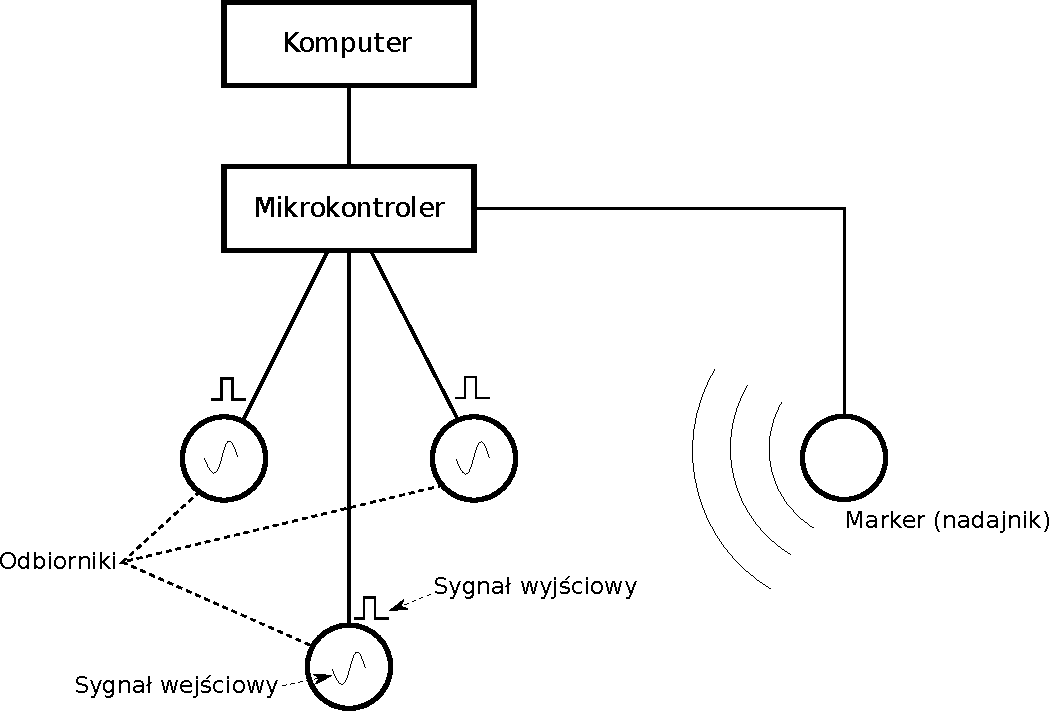
\includegraphics[width=\textwidth]{gfx/diagramy/schemat_blokowy_ukladu}
 \caption{Uproszczony schemat blokowy układu}
 \label{fig:device_scheme}
\end{figure}


\subsubsection{Po dłużce}
Działanie systemu opiera się o fakt\graffito{na fakcie?}, że dźwięk w powietrzu rozchodzi się ze stałą, znaną szybkością.

Ponieważ szybkość ta jest stała, można łatwo wyznaczyć odległość, jaką musiał przebyć dźwięk, aby dotrzeć do odbiornika:

\begin{equation}
 x = v \cdot t
 \label{eq:sound_distance}
\end{equation}
gdzie:\graffito{dodać informację nt. kalibracji - zmiana protokołu na obsługę potwierdzeń, oczekiwanie mikrokontrolera na potwierdzenie, rozpoczynanie kalibracją, wymóg piramidki do kalibracji}
\begin{description}
 \item[$x$] \ppauza~odległość przebyta przez dźwięk,
 \item[$v$] \ppauza~szybkość dźwięku w powietrzu,
 \item[$t$] \ppauza~czas od wysłania sygnału do jego dotarcia do odbiornika. 
\end{description}

Dane, jakie przekazywane są do komputera w celu dalszej obróbki zawierają, poza specyfikacją protokołu, tylko i wyłącznie odczyty z licznika dla każdego z odbiorników.

\paragraph{Przetwarzanie danych}
Aby dane były do czegoś użyteczne, wymagane jest ich przetworzenie. Przetwarzanie danych tej postaci może odbywać się różnorakimi metodami, np.:
\begin{itemize}
 \item rozpoznawanie gestów za pomocą sieci neuronowych,
 \item odtworzenie pozycji markera w trzech wymiarach,
 \item oczekiwanie na przemieszczenie markera do predefiniowanej pozycji,
 \item wiele innych.
\end{itemize}

\paragraph{Odtworzenie pozycji markera}
W celach demonstracyjnych postanowiłem pokazać, jak odtworzyć pozycję markera w trzech wymiarach korzystając tylko z informacji o względnym położeniu odbiorników oraz przekazywanych do komputera danych.
\newline
\newline
Ponieważ odbiorniki znajdują się w różnych, lecz znanych, położeniach w przestrzeni, odległość markera od każdego z nich może być różna.

Aby wyznaczyć położenie markera w trójwymiarowej przestrzeni, mając do dyspozycji odległości od każdego z odbiorników, należy założyć, że odbiorniki są środkami sfer, a promieniem każdej z nich \ppauza odległość, jaką przebył dźwięk od markera do tego odbiornika. Punkt przecięcia się tych sfer będzie pozycją markera.

\begin{figure}
  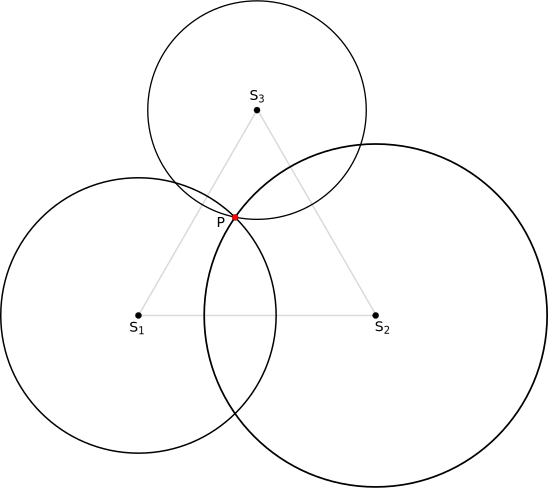
\includegraphics[width=\textwidth]{gfx/diagramy/schemat_przeciecia_sfer}
  \caption{Poglądowy schemat rozmieszczenia czujników}
  \label{fig:schema_spheres}
\end{figure}

\paragraph{Rozmieszczenie elementów}
Rysunek \ref{fig:schema_spheres}\graffito{W rysunku przyjęto widok ,,od przodu'', tzn. zachodzi $z = 0$ dla wszystkich elementów z wyjątkiem punktu $P$} prezentuje rozmieszczenie odbiorników na płycie testowej. Znajdują się one w punktach oznaczonych odpowiednio jako $S_1$, $S_2$ i $S_3$. Punkt $P$ to punkt przecięcia się sfer.

Ponieważ zastosowano tylko trzy odbiorniki, muszą one leżeć w jednej płaszczyźnie. Powoduje to, że będą istniały dokładnie dwa punkty przecięcia wspomnianych powyżej sfer \ppauza lustrzane do siebie względem płaszczyzny, w której znajdują się odbiorniki.\graffito{dodać notatkę w testach o możliwości wyeliminowania tego 'defektu' poprzez dodanie 4-tego odbiornika, niewspółpłaszczyznowego, jednak spowoduje to wzrost kosztów obliczeń}

Należy wziąć pod uwagę fakt, że zarówno marker jak i odbiorniki są urządzeniami ,,kierunkowymi'', umieszczonymi w tulejach, które powodują, że sygnał nie jest wysyłany dookólnie, lecz w pewnym \ppauza z grubsza określonym \ppauza kierunku, zaś amplituda sygnału odbieranego będzie większa, jeśli będzie on wpadał w tuleję, przez co szansa uznania go za poprawny jest znacznie większa.\graffito{sygnał dochodzący z boku może być ze słaby, aby został wyłapany}

Ta cecha układu została wykorzystana poprzez przeznaczenie układu do noszenia na tułowiu \ppauza łatwo zauważyć, że użytkownikowi ciężko byłoby przesunąć marker zbyt daleko do tyłu, gdyż ograniczałyby go stawy. 

Wykorzystując fakt, że człowiek trzyma ręce w większości przypadków przed sobą, szczególnie jeśli zamierza coś nimi robić, można spokojnie odrzucić jeden z punktów \ppauza ten który znajduje się ,,z tyłu''.

Ważnym\graffito{na pewno ważnym?} spostrzeżeniem jest dostrzeżenie, że aby wszystkie trzy sfery posiadały punkt\graffito{tutaj są pewne ograniczenia - jeśli zwiększymy promien jednej ze sfer, to możemy nie dostać punktu wspólnego dla wszystkich trzech sfer}, w którym będą się stykać, stykiem każdej pary sfer musi być okrąg\graffito{okrąg - w odróżnieniu od punktu lub braku styku}.

\paragraph{Trilateracja}
Metoda wyznaczenia trójwymiarowej pozycji znając odległości od trzech punktów o znanych współrzędnych nazywana jest \textit{trilateracją}\graffito{dodać info skąd to wiadomo}.

Problem wyznaczenia położenia markera można uprościć, przyjmując określony układ współrzędnych, w którym jeden z odbiorników znajduje się w początku układu współrzędnych, jeden na osi $x$, a trzeci pozostaje ,,swobodny''\graffito{Współrzędna $z$ dla wszystkich odbiorników równa jest~$0$}. Przyjmując takie rozmieszczenie, jakie zaprezentowane jest na rysunku \ref{fig:schema_coordinates}, odbiorniki mają współrzędne odpowiednio:
\begin{center}
 $S_1 (0, 0)$

 $S_2 (a, 0)$

 $S_3 (b, c)$
\end{center}

\begin{figure}
  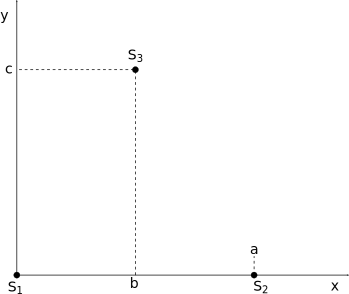
\includegraphics[width=\textwidth]{gfx/diagramy/schemat_uklad_wspolrzednych_clipped}
  \caption{Obrany układ współrzędnych}
  \label{fig:schema_coordinates}
\end{figure}

Równanie sfery ze środkiem w punkcie o współrzędnych $(x_0, y_0, z_0)$ i promieniu $r$ przyjmuje postać:

\begin{equation}
 r = \sqrt{(x - x_0)^2 + (y - y_0)^2 + (z - z_0)^2}
 \label{eq:sphere}
\end{equation}

Podstawiając do równania \ref{eq:sphere} współrzędne punktów $S_1$, $S_2$ i $S_3$ otrzymujemy następujący układ równań:

\begin{equation}
 \begin{cases}
  r_1 = \sqrt{x^2 + y^2 + z^2} \\
  r_2 = \sqrt{(x - a)^2 + y^2 + z^2} \\
  r_3 = \sqrt{(x - b)^2 + (y - c)^2 + z^2}
 \end{cases}
 \label{eq:sphere_system_1}
\end{equation}
gdzie $r_1$, $r_2$ i $r_3$ to odpowiednio odległości markera od każdego z odbiorników \textsmaller{\#1}, \textsmaller{\#2} i \textsmaller{\#3}, a zarazem promienie sfer, których punktu przecięcia poszukujemy.

W celu uproszczenia następnych obliczeń przyjmijmy poniższą postać równania \ref{eq:sphere_system_1}\graffito{należy pamiętać, że promień jest zawsze nieujemny}:
\begin{equation}
 \begin{cases}
  r_1^2 = x^2 + y^2 + z^2 \\
  r_2^2 = (x - a)^2 + y^2 + z^2 \\
  r_3^2 = (x - b)^2 + (y - c)^2 + z^2
 \end{cases}
 \label{eq:sphere_system_2}
\end{equation}

Rozwińmy najpierw drugie równanie z układu \ref{eq:sphere_system_2}:
\begin{equation}
 r_2^2 = (x - a)^2 + y^2 + z^2 = x^2 - 2xa + a^2 + y^2 + z^2
\end{equation}

Następnie odejmijmy je od równania pierwszego z systemu \ref{eq:sphere_system_2}:
\begin{equation}
 r_1^2 - r_2^2 = x^2 + y^2 + z^2 - (x^2 - 2xa + a^2 + y^2 + z^2) = 2xa - a^2
 \label{eq:determine_x_1}
\end{equation}

Z równania \ref{eq:determine_x_1} można łatwo wyznaczyć $x$:

\begin{eqnarray}
 r_1^2 - r_2^2 = 2xa - a^2 & | & + a^2\\
 r_1^2 - r_2^2 + a^2 = 2xa & | & \colon 2a\\
 x = \frac{r_1^2 - r_2^2 + a^2}{2a} \label{eq:determine_x_2}
\end{eqnarray}
\graffito{jak zapisać działanie wykonywane stronami?}

Podstawiając $x$ z równania \ref{eq:determine_x_2} do pierwszego równania układu \ref{eq:sphere_system_2} dowiemy się, który punkty są wspólne dla sfer mających środki w odpowiednio\graffito{przecinki?} $S_1$ i $S_2$:

\begin{eqnarray}
 r_1^2 = x^2 + y^2 + z^2 \\
 r_1^2 = \left(\frac{r_1^2 - r_2^2 + a^2}{2a}\right)^2 + y^2 + z^2 \\
 y^2 + z^2 = r_1^2 - \left(\frac{r_1^2 - r_2^2 + a^2}{2a}\right)^2 \label{eq:intersection_circle}
\end{eqnarray}

W równaniu \ref{eq:intersection_circle} prawa strona jest stała, widać więc, że jest to równanie okręgu.

Rozwińmy teraz równanie trzeciej sfery:

\begin{eqnarray}
 r^2_3 & = & (x - b)^2 + (y - c)^2 + z^2 \label{eq:third_sphere} \\
       & = & x^2 - 2bx + b^2 + y^2 - 2cy + c^2 + z^2 \nonumber
\end{eqnarray}

Podstawiając równanie pierwszej sfery przekształcone do postaci
\begin{equation*}
 y^2 + z^2 = r_1^2 - x^2
\end{equation*}
do wzoru \ref{eq:third_sphere} otrzymujemy:

\begin{eqnarray}
r_3^2 & = & x^2 - 2bx + b^2 - 2cy + c^2 + r_1^2 - x^2 \label{eq:third_sphere_substituted} \\
      & = & -2bx + b^2 - 2cy + c^2 + r_1^2 \nonumber
\end{eqnarray}

Na podstawie równania \ref{eq:third_sphere_substituted} można wyznaczyć $y$:

\begin{eqnarray}
 r_3^2 = -2bx + b^2 - 2cy + c^2 + r_1^2 & | & +2cy - r_3^2 \\
 2cy = -2bx + b^2 + c^2 + r_1^2 - r_3^2 & | & \colon 2c \\
 y   = \frac{-2bx + b^2 + c^2 + r_1^2 - r_3^2}{2c} \label{determine_y}
\end{eqnarray}

Ponieważ $x$ jest stałe\graffito{stałe i znane?}, jak pokazuje równanie \ref{eq:determine_x_2}, to prawa strona równania \ref{determine_y} również będzie stała.

Do wyznaczenia pozostało jeszcze jedynie $z$. Aby policzyć jego wartość, weźmy wzór pierwszej sfery z układu \ref{eq:sphere_system_1}, stąd $z$ będzie wynosić:
\begin{equation}
 z = \pm\sqrt{r_1^2 - x^2 - y^2}
\end{equation}

Jak jednak pamiętamy z opisu, jeden z tych punktów, ,,tylny'' odrzucamy, w związku z czym $z$ ostatecznie przyjmuje postać:
\begin{equation}
 z = \sqrt{r_1^2 - x^2 - y^2}
\end{equation}

Reasumując, jeśli przyjąć rozmieszczenie odbiorników takie jak na rysunku~\ref{fig:schema_coordinates}, punkt przecięcia się sfer\graffito{Dla uproszczenia przyjmujemy, że punkt taki zawsze istnieje, co w skonstruowanym systemie jest prawdziwe} będzie miał następujące współrzędne:

\begin{eqnarray}
 x & = & \frac{r_1^2 - r_2^2 + a^2}{2a} \\
 y & = & \frac{-2bx + b^2 + c^2 + r_1^2 - r_3^2}{2c} \\
   & = & \frac{-b\frac{r_1^2 - r_2^2 + a^2}{a} + b^2 + c^2 + r_1^2 - r_3^2}{2c} \nonumber \\
 z & = & \sqrt{r_1^2 - x^2 - y^2} \\
   & = & \sqrt{r_1^2 - \left(\frac{r_1^2 - r_2^2 + a^2}{2a}\right)^2 - \left(\frac{b\frac{r_1^2 - r_2^2 + a^2}{-a} + b^2 + c^2 + r_1^2 - r_3^2}{2c}\right)^2} \nonumber
\end{eqnarray}



W celu pomiaru różnicy czasów zdecydowałem się wykorzystać ośmiobitowy timer/counter dostępny w używanym mikrokontrolerze.\graffito{to musi iść gdzieś indziej}

\section{Oprogramowanie}
\subsection{Wykresy}
W celach demonstracji działania stworzyłem program, który pokazuje dane odczytane z urządzenia w dwóch postaciach:
\begin{itemize}
 \item dane odczytane \ppauza rysowany jest wykres danych, jakie zostały wysłane przez urządzenie,
 \item dane przetworzone \ppauza rysowany jest wykres prezentujący pozycję wybranego markera w trzech wymiarach.
\end{itemize}

\myChapter{Implementacja}\label{ch:implementation}
%************************************************

Jako zwolennik wolnego i otwartego oprogramowania starałem się korzystać tylko i wyłącznie z takich właśnie narzędzi.

\section{Oprogramowanie mikrokontrolera}
W pracy wykorzystany został układ \textsmaller{AVR Atmega8}, będący ośmiobitowym mikrokontrolerem. Sprzęt ten znacznie różni się od architektury znanej z komputerów osobistych \spacedallcaps{PC} i choć sama idea programowania jest podobna, wszystko pozostawione jest programiście, co w połączeniu z koniecznością programowania na bardzo niskim poziomie, jaki nie jest promowany na studiach, stanowi dodatkowe wyzwanie.

Oprogramowanie zostało stworzone w języku \texttt{C}, wykorzystując do kompilacji kompilator \textsmaller{avr-gcc} oraz bibliotekę \textsmaller{avr-libc}. Do programowania wykorzystałem program \textsmaller{avrdude}

\subsection{Wymagania}
Zadaniem tej części oprogramowania jest dostarczenie danych, których obróbką zajmie się komputer. Wymagania, jakie są stawiane to przede wszystkim:
\begin{itemize}
 \item zwięzłość \ppauza program ma robić tylko i wyłącznie to, co absolutnie konieczne, ponieważ wprowadzanie dodatkowego, nadmiarowego kodu będzie powodowało opóźnienia w działaniu, co może przekładać się na
    niestabilność działania,
 \item dokładność \ppauza dostarczanie niepewnych danych mija się z celem pracy, należy więc zadbać o to, aby dane były możliwie najdokładniejsze,
 \item prostota \ppauza ze względu na niewielkie możliwości mikrokontrolera \ppauza w porównaniu do komputerów \ppauza trzeba zoptymalizować wszelkie używane struktury i unikać wykonywania pracy, którą spokojnie może zająć się komputer.
\end{itemize}

Uważam, że program, który napisałem spełnia wszystkie stawiane mu wymagania. Mieści się w niecałych 200 liniach \ppauza nie ma zbędnego kodu, dba o poprawne inicjalizowanie \index{timer}timerów urządzenia \ppauza stara się o dokładność danych, posiada możliwie najmniejsze struktury, które pozwolą przechować dane.

Należy zauważyć, że obrany rozmiar zmiennych, t.j. 8 bitów, został dopasowany do rozmiaru rejestrów mikrokontrolera. W przypadku zmiennych o długości 16 bitów znacznie wzrasta ilość taktów zegara, podczas których dane te są przetwarzane. Krótkie zmienne pozwalają na przechwycenie danych timera \ppauza rejestru \texttt{TCNT0} oraz licznika przepełnień \texttt{ovfCounter}\graffito{Rejestr \texttt{TCNT0} przechowuje aktualny stan licznika, a zmienna \texttt{ovfCounter} ilość cykli timera.} \ppauza w jednym takcie zegara.

Mikrokontroler posiada również drugi, szesnastobitowy timer, którego użycie pozwoliłoby na zwiększenie dokładności, wiązałoby się jednak z mankamentem wspomnianym powyżej, zaś dokłądność osiągana przez oprogramowanie wykorzystujące timer o wielkości ośmiu bitów, jaka została opisana w sekcji \ref{section:microcontroller_limit}, jest wystarczająca do bardzo dokładnego śledzenia pozycji.

\subsection{Dokładność}\label{section:precision}
\paragraph{Ograniczenia mikrokontrolera}
\label{section:microcontroller_limit}

Dokładność, jaką można uzyskać za pomocą ośmiobitowego timera pracującego w układzie taktowanym zegarem $F_{cpu} = 8$ MHz wyznacza się w następujący sposób:\graffito{znając częstotliwość wykorzystanego sygnału dźwiękowego należy poznać jego okres $T$ i porównać z danymi z wyliczeń mikrokontrolera w celu określenia co jest ogranicznikiem}
\begin{enumerate}
 \item \index{prescaler}prescaler\graffito{prescaler - wytłumaczyć} ustawiony jest na $F_{cpu}/8$, należy poznać interwał $i$, co jaki wyzwalane będzie przerwanie timera:
    \begin{equation}
      i = \frac{1}{F_{cpu}/8} = \frac{1}{1~\textrm{MHz}} = 0,000001~\textrm{s} = 0,001~\textrm{ms} = 1~\mu\textrm{s}
      \label{eq:sampling_frequency}
    \end{equation}

 \item znając interwał $i$ oraz szybkość dźwięku w powietrzu $v$, wyznaczyć należy drogę, jaką przebędzie dźwięk w czasie $i$, wykorzystując w tym celu wzór~\ref{eq:sound_distance}:
    \begin{equation}
      x = v \cdot i = 340~\frac{\textrm{m}}{\textrm{s}} \cdot 1~\mu\textrm{s} = 0,34~\textrm{mm}
      \label{eq:microcontroller_limit}
    \end{equation}
\end{enumerate}

Jak pokazuje równanie~\ref{eq:microcontroller_limit}, teoretyczna dokładność sprzętu jest bardzo duża i znacznie przekracza wymagania gier wideo, gdzie w centrum zainteresowania są żwawe, gwałtowne ruchy. Pozwoli to na wykorzystanie układu w zastosowaniach wymagających większej precyzji, jak np. modelowanie trójwymiarowe lub wizualizacja danych medycznych.

Ponieważ \index{timer}timer ma tylko osiem bitów, należy spodziewać się, że nastąpi jego przepełnienie zanim zostanie odczytane wygaszenie pinu. Przepełnienie wystąpi po dokładnie $2^8 = 256$ aktualizacjach timera. Zajmie to $256 \cdot 1~\mu\textrm{s} = 256~\mu\textrm{s}$, a dźwięk w tym czasie zdąży przebyć odległość 
\begin{equation}
 340~\frac{\textrm{m}}{\textrm{s}} \cdot 256~\mu\textrm{s} = 87,04~\textrm{mm}
\end{equation}

Rozdzielczość można dalej zwiększyć zmniejszając dzielnik \index{prescaler}prescalera \graffito{Zmiana ta musiałaby zostać odwzorowana w aplikacjach wykorzystujących ten interfejs sterowania komputerem} oraz zwiększając częstotliwość pracy mikrokontrolera.

\paragraph{Ograniczenia markerów}
\label{section:sound_limit}

Ze względu na wykorzystanie nadajników i odbiorników ultradźwiękowych używających dźwięku o częstotliwości $F_{d} = 40$ kHz, należy zbadać jakie narzuca to ograniczenia.

Podobnie jak w przypadku wyliczania ograniczeń mikrokontrolera, tak i w tym przypadku należy wyznaczyć minimalny interwał, w jakim może zajść zmiana.

Za zmianę będziemy przyjmować wygaszenie pinu mikrokontrolera, co spowodowane jest zaniknięciem nadawanego sygnału. Zdarzenie takie może zajść jedynie co pełny okres fali dźwiękowej. Policzmy więc odległość, jaka będzie dzieliła obraną fazę fali w dwóch ,,sąsiadujących'' okresach:

\begin{enumerate}
 \item wyliczamy okres $T$ fali dźwiękowej:
    \begin{equation}
      T = \frac{1}{F_d} = \frac{1}{40~\textrm{kHz}} = 0,000025~\textrm{s} = 0,025~\textrm{ms} = 25~\mu\textrm{s}
    \end{equation}
 \item znając $T$ skorzystajmy ponownie ze wzoru~\ref{eq:sound_distance}:
    \begin{equation}
      x = v \cdot T = 340~\frac{\textrm{m}}{\textrm{s}} \cdot 25~\mu\textrm{s} = 8,5~\textrm{mm}
      \label{eq:sound_limit}
    \end{equation}
\end{enumerate}

\paragraph{Ograniczenia całego systemu}
Jak pokazują obliczenia przeprowadzone w paragrafach~\nameref{section:microcontroller_limit} i~\nameref{section:sound_limit}, głównym ograniczeniem dokładności bieżącej wersji systemu jest wykorzystanie ,,powolnych'' nadajników i odbiorników.

Zdecydowałem się na wykorzystanie elementów \graffito{Należy spodziewać się, że czujniki stosowane np. w aparturze USG jest odpowiednio droga, wykorzystuje jednak znacznie wyższe częstotliwości} o takich właśnie charakterystykach, ponieważ są to jedyne dostępne na rynku, których cena pozwala na ukończenie projektu.

Aby zwiększyć dokładność urządzenia należałoby wymienić nadajniki i odbiorniki na podobne modele, korzystające z wyższych częstotliwości, a także wymienić kwarc generujący częstotliwość dla tych elementów. Bez konieczności przeprogramowywania mikrokontrolera można zastosować elementy używające częstotliwości do
\begin{equation}
 f = \frac{1}{i} = \frac{1}{1~\mu\textrm{s}} = 1~\textrm{MHz}
\end{equation}
gdyż jest to częstotliwość próbkowania określona wzorem \ref{eq:sampling_frequency}\graffito{dodać info o możliwości podkręcenia częstotliwości przez zmniejszenie delay-ów oraz wysyłanie tylko impulsu, zamiast ciągłego sygnału, ponadto używanie w otwrtych przestrzeniach}.

\subsection{Algorytm}
Oprogramowanie zapisane w pamięci mikrokontrolera steruje markerami i odbiornikami w następujący sposób:\graffito{metoda wyznaczania }
\begin{enumerate}
 \item \index{prescaler}prescaler urządzenia jest resetowany,\label{enum:prescaler}
 \item uruchamiany jest wewnętrzny licznik urządzenia,
 \item wysyłany jest sygnał, który aktywuje jeden z dwóch markerów, powoduje to rozpoczęcie nadawania sygnału przez ten marker,
 \item następuje aktywne oczekiwanie na ,,wygaszenie''\graffito{opisać czym jest wygaszenie} pinów wszystkich odbiorników,\graffito{Czas wygaszenia każdego z pinów (różnica czasu pomiędzy rozpoczęciem nadawania i odebrania sygnału z danego odbiornika) jest zapamiętywany}
 \item zatrzymywany jest wewnętrzny timer urządzenia,
 \item dane o odstępach czasowych przekazywane są do komputera,
 \item następuje uśpienie układu, które pozwala na zaniknięcie sygnałów ultradźwiękowych,
 \item cała operacja powtarzana jest dla drugiego markera.
\end{enumerate}
Algorytm ten obrazuje diagram przedstawiony na rysunku \ref{fig:firmware_sequence_diagram}.

\begin{figure}
 % fugly hack
 \hspace{-10em}
 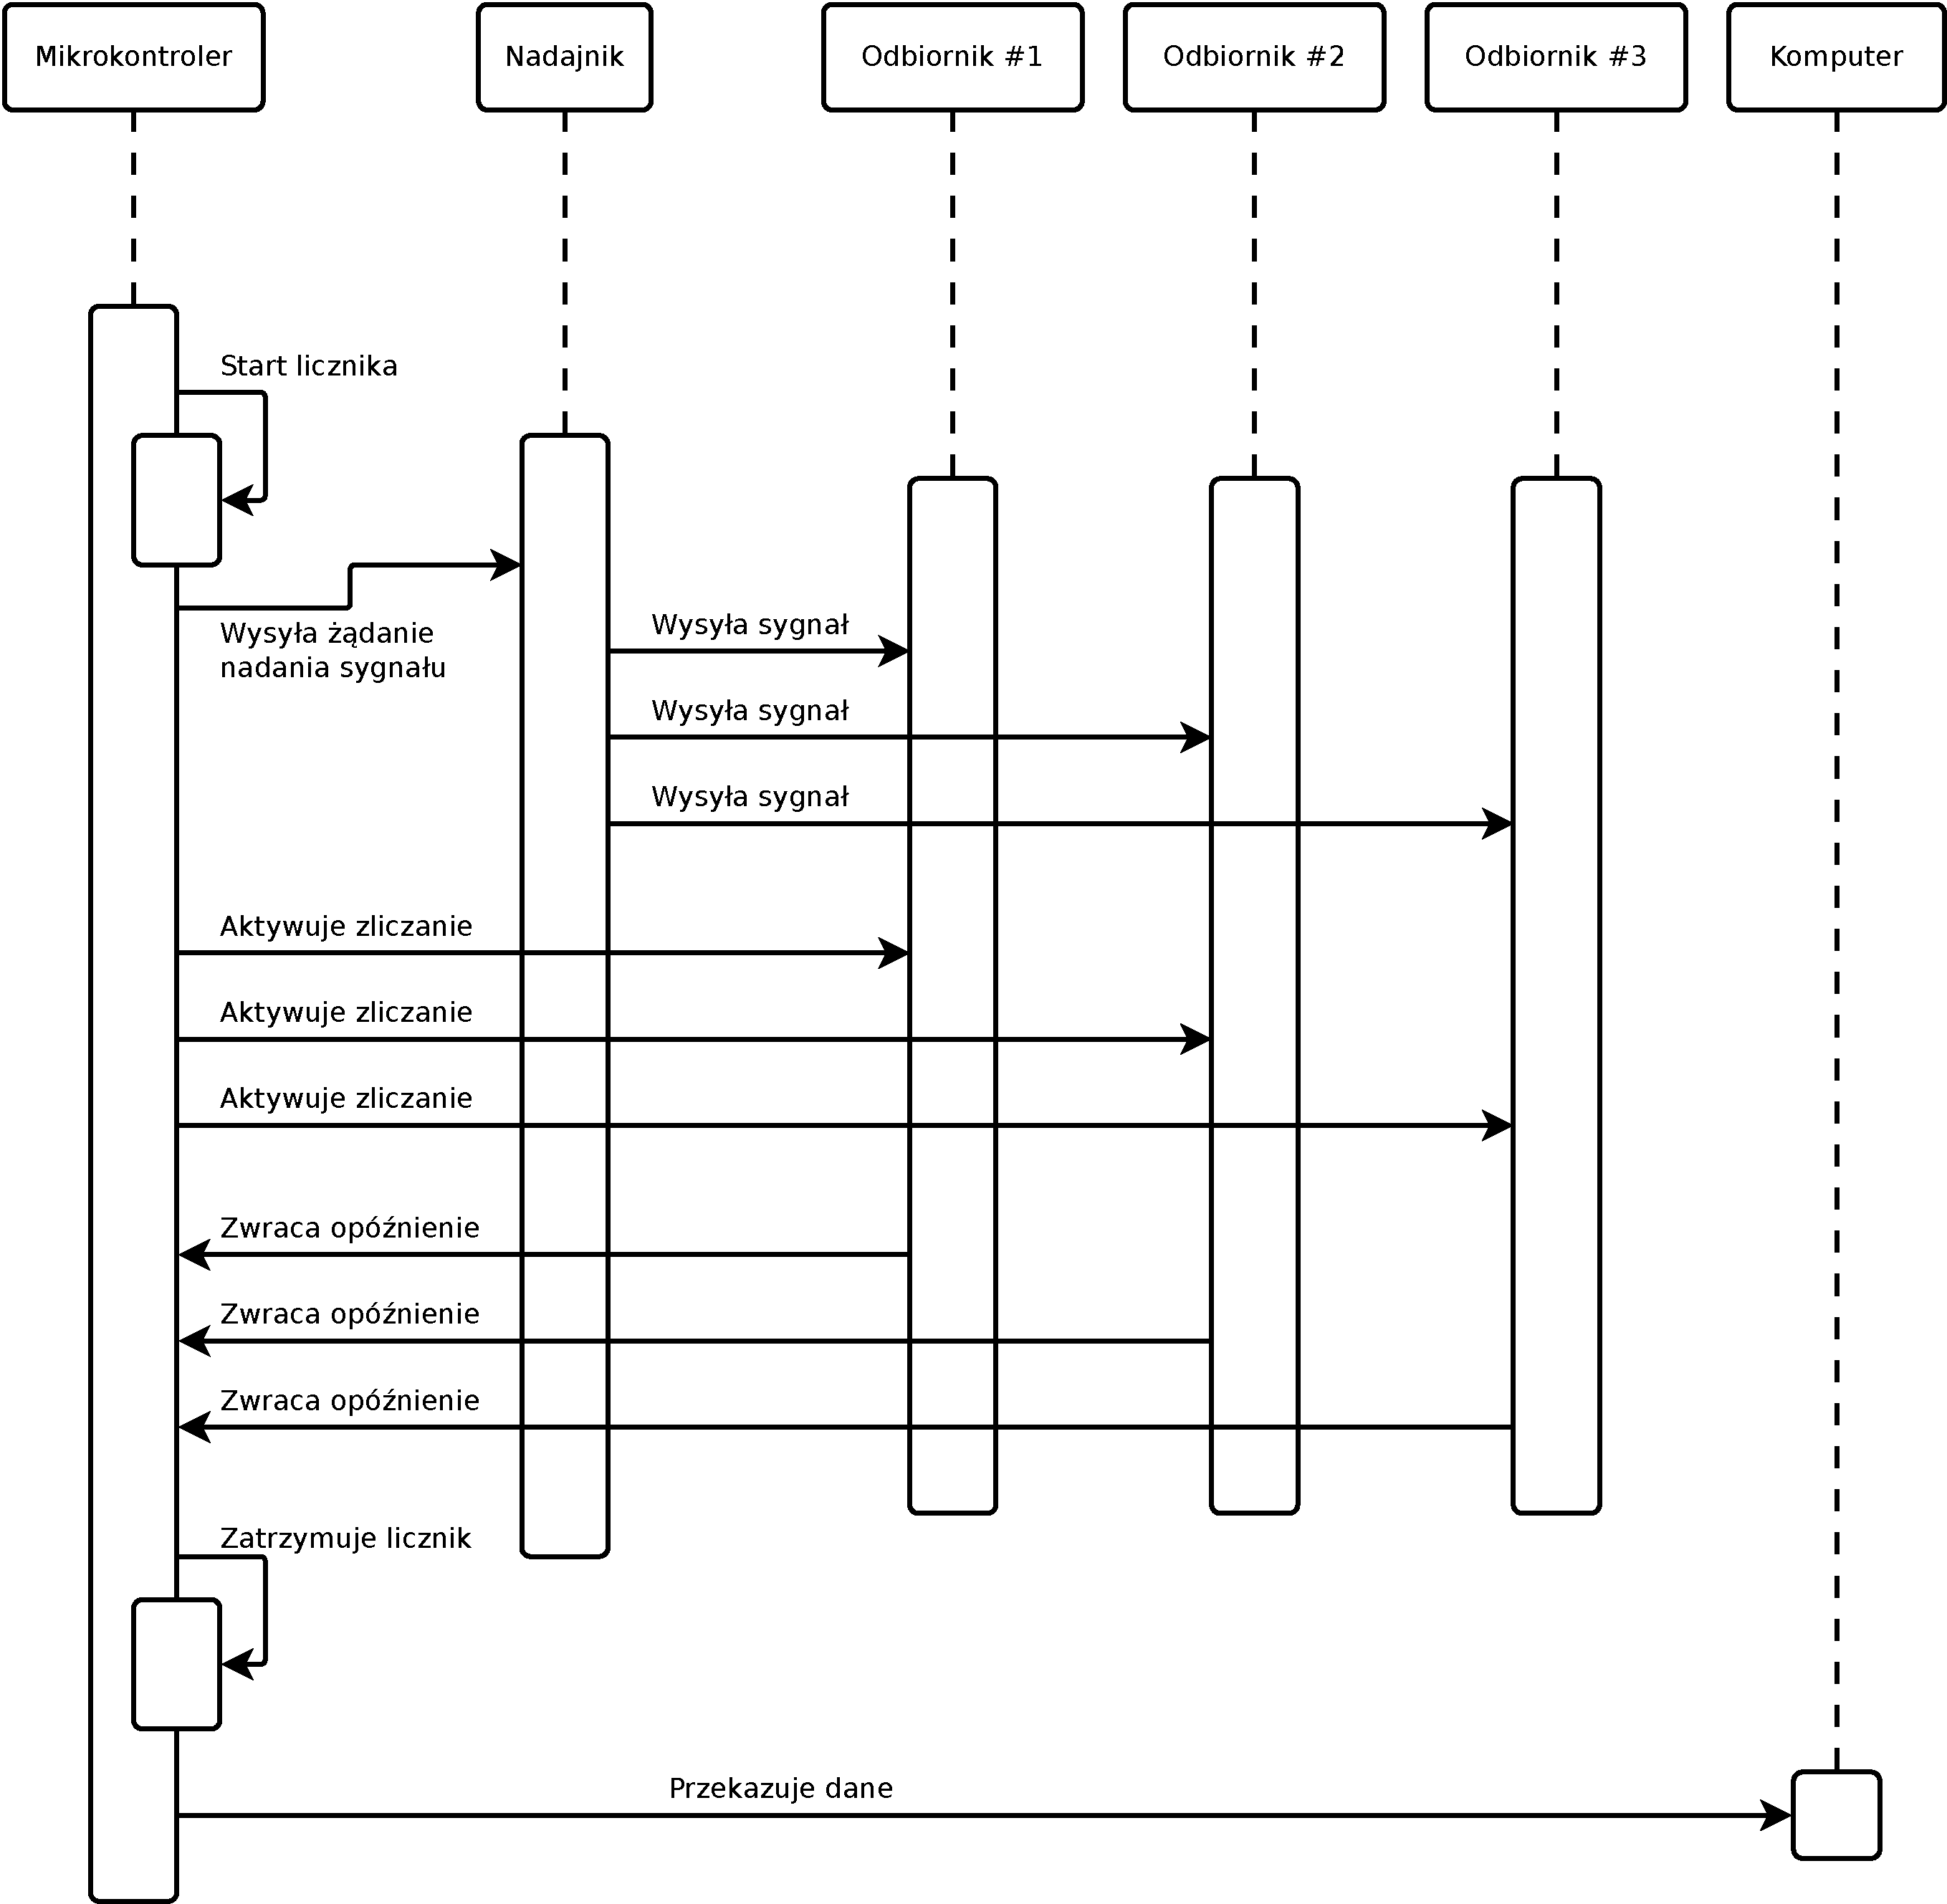
\includegraphics[width=45em]{gfx/diagramy/diagram_sekwencji_sprzetu.pdf}
 \caption{Diagram sekwencji oprogramowania mikrokontrolera}
 \label{fig:firmware_sequence_diagram}
\end{figure}

\paragraph{Prescaler}
W mikrokontroler wbudowany jest \index{prescaler}\textsl{prescaler}, czyli dzielnik częstotliwości, o programowanym stopniu podziału. Jego działanie polega na zliczaniu taktów zegara; gdy wewnętrzny licznik prescalera osiągnie zaprogramowaną wcześniej wartość, wyzwalane jest przerwanie timera oraz następuje przepełnienie licznika, w związku z czym zliczana wartość ,,przekręca się'' i liczenie rozpoczyna się ponownie od zera.

Punkt \ref{enum:prescaler} algorytmu jest bardzo istotny, gdyż nie ma możliwości\graffito{Nawet gdyby możliwość odczytania tej wartości istniała, działanie to wprowadzałoby niepożądane opóźnienia} sprawdzenia aktualnego stanu licznika prescalera, natomiast rozpoczęcie odliczania może nastąpić w dowolnym momencie czasu, przez co może być niekoniecznie zsynchronizowane z wyzwoleniem przerwania przez prescaler, efektem czego byłyby pomiary, które charakteryzowałyby się pewną zmienną niedokładnością.

\paragraph{Przerwania}
W działaniu programu dużą rolę odgrywają procedury obsługi przerwań (ang. \textsl{ISR \ppauza Interrupt Service Routine}). Są to krótkie fragmenty kodu, które wywoływane są przez mikrokontroler w przypadku zajścia pewnego zdarzenia. Ich użycie pozwala na pewien stopień ,,wielowątkowości'', gdyż (w zależności od ustawienia flag) mogą one przerwać wykonywanie głównego toku programu do momentu, aż przerwania nie zostaną ,,obsłużone'', tzn. instrukcje zawarte w procedurze ISR nie zostaną wykonane.

Implementacja procedur obsługi przerwań jest rozszerzeniem języka C, która jest charakterystyczna dla wykorzystanej rodziny układów i wykorzystanego kompilatora, co powoduje, że wykorzystanie innego kompilatora lub innej rodziny układów wymaga przepisania procedur ISR zgodnie z nowymi wymaganiami.

Jednym z wykorzystanych przerwań jest przerwanie wywoływane przez moduł \texttt{Timer/Counter0}: \texttt{Timer/Counter0 Overflow} (\texttt{TOV0}). Jest ono wyzwalane, gdy licznik \texttt{TCNT0} przekroczy maksymalną możliwą dla niego wartość i rozpocznie się ponowne odliczanie od zera. Zadaniem zawartego w tej procedurze kodu jest tylko i wyłącznie inkrementacja zmiennej \texttt{ovfCounter}, dzięki czemu znana jest ilość przepełnień licznika. W przypadku pominięcia tej danej, pomiary ograniczony byłyby do zaledwie 256 możliwości odległości markera od odbiornika.

Drugie wykorzystane przerwanie jest również przerwaniem licznika i wyzwalane jest przez moduł \texttt{Timer/Counter1}. Jedynym zadaniem tego przerwania jest obsługa jednej z diod, której zadaniem jest wizualne potwierdzenie sprawności i działania układu.

Przykład procedury obsługi przerwania na podstawie opisanej właśnie funkcjonalności prezentuje poniższy listing:

\lstinputlisting[caption=Procedura obsługi przerwania \texttt{Timer/Counter0 Overflow}, title=Procedura obsługi przerwania \texttt{Timer/Counter0 Overflow}]{testy/atmega_interrupt.c}

Oznaczenie zmiennej jako \texttt{volatile} oznajmia kompilatorowi, że wszelkie odczyty i zapisy muszą operować na wartości zmiennej z pamięci. W przypadku braku takiego zapisu kompilator podczas kompilowania kodu źródłowego z włączoną flagą optymalizacji może przyjąć, że procedura zmieniająca wartość zmiennej nie jest nigdzie wywoływana, przez co bezpiecznym jest cache-owanie wartości zmiennej, a w efekcie zignoruje skutki wywołania przerwania.

Makro \texttt{ISR(vector [, attributes])} z biblioteki \textsmaller{avr-libc} definiuje następujące po nim ciało funkcji jako procedurę obsługi przerwania. Argument \texttt{vector} jest wymagany i oznacza pozycję w wektorze przerwań mikrokontrolera, do której przypisany ma zostać kod. Argument \texttt{attributes} jest opcjonalny i modyfikuje działanie procedury ISR.

Wygenerowany wektor przerwań, prezentujący obecność tylko dwóch, wymienionych powyżej, procedur obsługi przerwania prezentuje poniższy listing:

\lstinputlisting[caption=Wektor obsługi przerwań, title=Wygenerowany wektor obsługi przerwań]{testy/interrupt_vector.txt}

Pierwsza pozycja na liście jest punktem wejścia programu, od którego rozpoczyna się wykonywanie kodu. Pozycje z adresów \texttt{0x10} i \texttt{0x12} to przekierowania do odpowiednio procedur ISR dla przerwań \texttt{Timer/Counter0 Overflow} i \texttt{Timer/Counter1 Overflow}.

\section{Oprogramowanie dla komputera}
\subsection{Trilaterator}
Pierwsza ze stworzonych aplikacji przeznaczona jest do przeprowadzania trilateracji, o której mowa w sekcji \ref{par:trilateration}. Wykonuje ona automatycznie obliczenia dane wzorami \ref{eq:trilateration_final_x}, \ref{eq:trilateration_final_y} i \ref{eq:trilateration_final_z}. Interfejs aplikacji umożliwia wprowadzanie wszelkich danych dotyczących rozmieszczenia odbiorników jak i markera.

Aplikację prezentuje rysunek \ref{fig:trilaterator}.

\begin{figure}[p]
 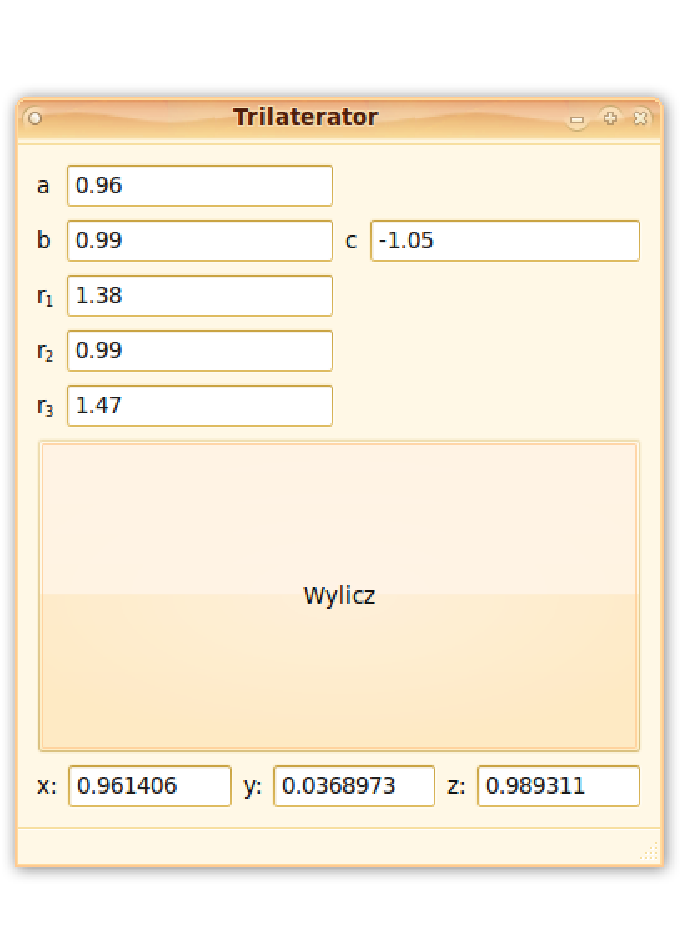
\includegraphics[width=\textwidth]{gfx/trilaterator.pdf}
 \caption{Trilaterator. Aplikacja dokonująca trilateracji}
 \label{fig:trilaterator}
\end{figure}

\begin{figure}[p]
 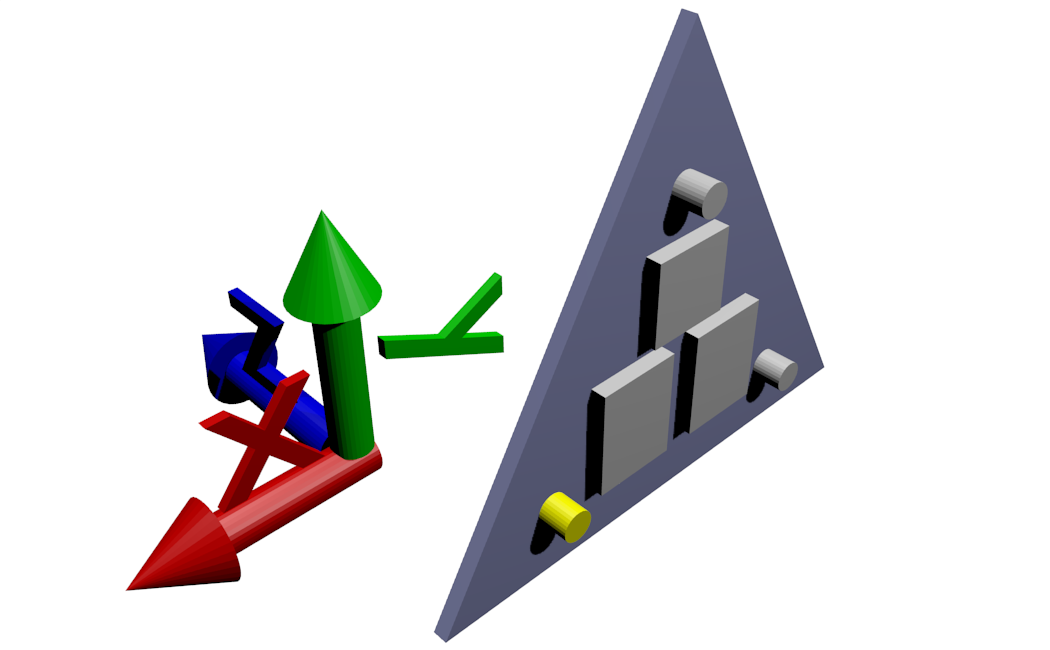
\includegraphics[width=\textwidth]{gfx/uklad_render.png}
 \caption[Model systemu i przyjęty układ współrzędnych]{Model systemu wraz z przyjętym układem współrzędnych. Układ ma swój początek w odbiorniku oznaczonym kolorem żółtym}
 \label{fig:coordinate_system}
\end{figure}

\subsection{Charter}
Kolejna aplikacja prezentująca możliwości systemu służy do rysowania wykresów w czasie rzeczywistym na podstawie danych pobranych z mikrokontrolera. Dla porównania dostępne są dwa rodzaje wykresów jednocześnie:
\begin{itemize}
 \item odległość od odbiornika \ppauza pokazuje odległość wybranego markera od każdego z odbiorników,
 \item położenie \ppauza dokonuje w locie trilateracji dla bieżącej próbki i rysuje wykres położenia wybranego markera w trzech wymiarach, zgodnie z układem odniesienia przedstawionym na rysunku \ref{fig:coordinate_system}.
\end{itemize}

Odległość od odbiorników podawana jest jako wartość licznika odczytana z mikrokontrolera. Aby dokonać konwersji na centymetry, należy (w oparciu o równanie \ref{eq:microcontroller_limit}) przeliczyć:
\begin{equation}
 d = \frac{x * 0,34\textrm{mm}}{10}
\end{equation}
gdzie:
\begin{description}
 \item[$d$] \ppauza~wyznaczona odległość w centymetrach,
 \item[$x$] \ppauza~odległość odczytana z wykresu.
\end{description}

Program dokonuje transformacji układu współrzędnych, aby w efekcie uzyskać układ pokazany na rysunku \ref{fig:coordinate_system}.

Jest to taki sam układ, jak wykorzystywany w bibliotece \textsc{OpenGL}, co znacząco ułatwia pracę, ponieważ nie jest wymagana żadna dodatkowa konwersja układu współrzędnych aby narysować pozycję markera.

\section{Protokół}
\label{sec:protocol}
\index{protokół}
Mikrokontroler komunikuje się z komputerem za pomocą standardu \index{RS232}\textsmaller{RS232}, do obsługi którego wykorzystuje moduł \index{USART}\textsmaller{USART}. Aby uzgodnić dane pomiędzy komputerem a mikrokontrolerem, zaprojektowałem protokół, zgodnie z którym następuje przekazanie danych.

Protokół taki powinien zawierać możliwie mało nadmiarowych danych, umożliwiać synchronizację bez względu na moment włączenia nadajnika (mikrokontrolera) względem odbiornika (komputera) oraz zawierać wszystkie potrzebne informacje do odtworzenia położenia wszystkich obsługiwanych markerów.

Mianem \index{raport}\emph{raportu} będziemy nazywać jeden pełen zestaw danych, jakie przesyła do komputera mikrokontroler.

Raport w zaprojektowanym protokole prezentuje rysunek \ref{fig:protocol}.

\begin{figure}
 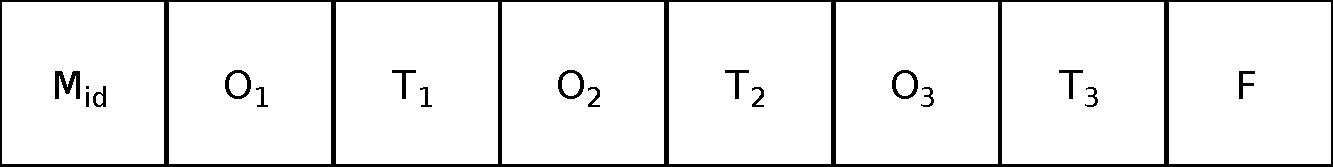
\includegraphics[width=\textwidth]{gfx/diagramy/protokol.pdf}
 \caption[Schemat raportu]{Raport w protokole komunikacji mikrokontrolera z komputerem}
 \label{fig:protocol}
\end{figure}

Każda ramka składa się z ośmiu bajtów, do których należą:
\begin{itemize}
 \item \texttt{M$_\textrm{\texttt{id}}$} \ppauza $id$ markera,
 \item \texttt{O$_n$} \ppauza wartość zmiennej \texttt{ovfCounter} w chwili wygaszenia pinu odbiornika $n$,
 \item \texttt{T$_n$} \ppauza wartość rejestru \texttt{TCNT0} w chwili wygaszenia pinu odbiornika $n$,
 \item \texttt{F} \ppauza zawsze \texttt{0xFF}.
\end{itemize}

Pole \texttt{F} wraz z polem \texttt{M$_\textrm{\texttt{id}}$} służy do synchronizacji danych odbieranych przez komputer. Metodę \index{synchronizacja}synchronizacji prezentuje algorytm \ref{alg:sync}.

\begin{algorithm}
\caption{Metoda synchronizacji danych}
\label{alg:sync}
\begin{algorithmic}[1]
  \REQUIRE \texttt{dane} \ppauza tablica dynamiczna, do której końca dopisywane są przychodzące dane
  \WHILE{\texttt{dane.count() $\geq$ 8}}
    \WHILE{\texttt{dane.count() $\geq$ 8 \&\& (dane[0] != M$_\textrm{\texttt{id}}$ \textbar{}\textbar{} dane[7] != 0x77})}
      \STATE usuń(\texttt{dane[0]})
    \ENDWHILE
  \ENDWHILE
\end{algorithmic}
\end{algorithm}

Należy zauważyć, że poza samymi danym protokołu, pomiędzy kompterem, a mikrokontrolerem przekazywane są również dane kontrolne standardu \index{RS232}RS232:
\begin{itemize}
  \item bity startu,
  \item bity stopu.
\end{itemize}

Zrezygnowałem natomiast z funkcji:
\begin{itemize}
 \item bity parzystości \ppauza te dane kontrolne bardzo słabo spełniają swoją rolę, gdyż są bardzo podatne na zakłócenia, które powodują przestawienie parzystej ilości bitów,
 \item kontrola przepływu \ppauza funkcjonalność nie jest dostępna w mikrokontrolerze.
 \item więcej niż 8 bitów w jednej ramce \ppauza chociaż mikrokontroler oferuje przesłanie do 9 bitów danych w jednej ramce, to wykorzystanie tej funkcjonalności znacznie ograniczyłoby funkcjonalność platformy ze względu na fakt, iż układy stosowane w komputerach rzadko kiedy oferują obsługę takich ramek\graffito{Obsługa 9-bitowych ramek wymaga też specjalnego oprogramowania}, ponadto spowodowałoby dodatkowy narzut pracy na mikrokontrolerze związany z podziałem danych na 9-bitowe części, nie oferując przy tym żadnego wzrostu wydajności \ppauza przesłanie 64 bitów wymagałoby i tak 8 ramek.
\end{itemize}

Pełna ramka standardu RS232 składa się zatem z 10 bitów:
\begin{enumerate}
 \item bit startu,
 \item 8 bitów danych,
 \item bit stopu.
\end{enumerate}
\myChapter{Testy}\label{ch:tests}
%************************************************

\section{Cele}

Głównym zadaniem przeprowadzonych testów było zbadanie zachowania stworzonego systemu i oprogramowania pod kątem wykorzystania w grach wideo\graffito{Wynika to ze studiowania na specjalności Technologii Gier i~Symulacji Komputerowych.}. Nie jest jednak trudno sobie wyobrazić inne dziedziny, w których można wykorzystać system, jak np.:
\begin{itemize}
 \item medycyna \ppauza manipulacja trójwymiarowymi obrazami skanów pacjentów,
 \item cyfrowe modelowanie \ppauza szybkie prototypowanie modeli,
 \item tworzenie filmów \ppauza przechwytywanie ruchu.
\end{itemize}

Głównym atutem systemu w tych dziedzinach jest naturalny sposób manipulacji i~interakcji z komputerem ze względu na pobieranie dodatkowo \ppauza w odróżnieniu od standardowego zostawu klawiatura + myszka \ppauza trzeciego wymiaru.

\section{Metody}
Aby określić przydatność systemu, należy zbadać kilka czynników. Ich wagi będą różnić się, w zależności od planowanego wykorzystania, jednak można zauważyć, że należy dążyć do optymalizacji cech takich jak:
\begin{itemize}
 \item dokładność,
 \item stabilność,
 \item niezawodność,
 \item prostota użytkowania,
 \item kompatybliność z oprogramowaniem,
 \item szybkość.
\end{itemize}


\section{Wyniki}
% dokladnosc
\paragraph{Dokładność}
Dokładność systemu została już określona w sekcji \ref{section:precision}, pozwolę więc sobie jedynie przytoczyć obliczone parametry.

Istnieją dwa rodzaje ograniczeń: spowodowane stworzonym oprogramowaniem oraz spowodowane wykorzystanym sprzętem. Ominięcie tych pierwszych jest stosunkowo łatwe\graffito{Trzeba liczyć się z~faktem, że można natknąć się na ograniczenia mikrokontrolera.} i~wymaga tylko zmiany pewnych parametrów oraz ponowne zaprogramowanie układu. W przypadku drugiego typu ograniczeń należy spodziewać się konieczności modyfikacji układu, jeśli chciałoby się zwiększać dokładność.

Mikrokontroler jest w stanie mierzyć pozycję markera z dokładnością do 0,34mm\graffito{Równania odpowiednio \ref{eq:microcontroller_limit}~i~\ref{eq:sound_limit}.}, natomiast wykorzystanie sygnałów ultradźwiękowych o częstotliowści 40kHz nakłada na system ograniczenie dokładności do 8,5mm, a zatem ograniczenie całego systemu wynosi 8,5mm.

Chociaż w wielu przypadkach taka dokładność jest zupełnie wystarczająca, pozostawia jednak trochę do życzenia.

% stabilnosc
\paragraph{Stabilność}
Pomimo przytoczonej powyżej, relatywnie małej, dokładności układ wykazuje pewną niestabilność, która objawia się drganiem odtworzonej pozycji \index{marker}markera. Widać to dobrze na rysunku \ref{fig:position_shaky}, którego górna część pokazuje odtworzoną pozycję w trzech wymiarach. Wszystkie dane, a w szczególności wartość $X$ oraz $Z$, wykazują kilkucentymetrowe drgania pomimo stabilnego umocowania zarówno układu jak i markera.

\begin{figure}
 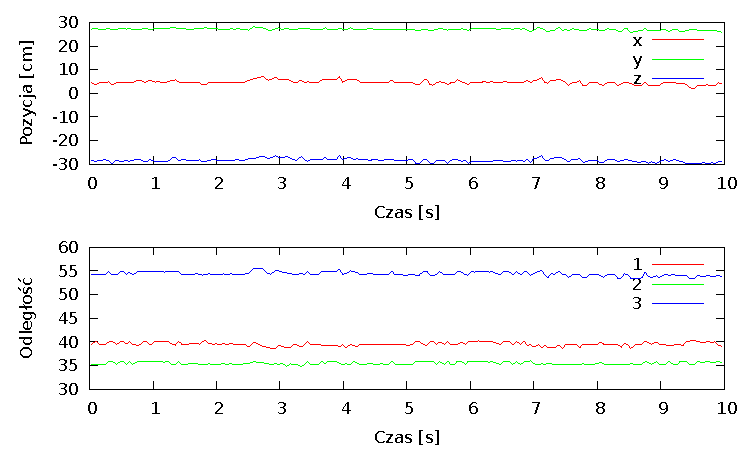
\includegraphics[width=\textwidth]{gfx/pozycja/pozycja.pdf}
 \caption[Wykres pozycji i odległości jednego z markerów]{Wykres pozycji i odległości od czujników jednego z~markerów w~stałej pozycji}
 \label{fig:position_shaky}
\end{figure}

% niezawodność
%\graffito{coś trzeba napisać o niezawodności}

% prostota użytkowania
\paragraph{Prostota użytkowania}
Starałem się zaprojektować system w~taki sposób, aby korzystanie z niego było możliwie proste, jednak wymogi systemu powodują, że korzystanie z niego nie jest tak proste, jak ma to miejsce w przypadku systemów ,,konkurencyjnych'' \graffito{Wiimote, Sixaxis, Kinect...}.

Aby móc w pełni wykorzystać oprogramowanie, a~w~szczególności program \textsmaller{\nameref{sec:app_stickman}}, wymagane jest dokonanie \index{kalibracja}kalibracji. Nie jest to czynność trudna, lecz wymóg wykonania jej każdorazowo po uruchomieniu może zniechęcać użytkowników.

Kalibracja ma na celu ustawienie wewnętrznych parametrów programu, które będą pozwalały na dokładniejsze odwzorowanie ruchów użytkownika. Na wykorzystywane parametry składają się długość ręki, pozycja ramienia i rotacja ramienia.

W zależności od trybu kalibracji wymagane jest pobranie dwóch lub trzech punktów kontrolnych; w tym celu należy:
\begin{enumerate}
 \item jeśli została już dokonana kalibracja od uruchomienia programu, należy ją zresetować za pomocą stosownego przycisku,
 \item ustawić rękę (marker) w ustalonej pozycji względem ciała,
 \item nacisnąć przycisk informujący program o ustawieniu markera,
 \item powtórzyć czynność dla pozostałych punktów kontrolnych,
 \item gdy zostaną pobrane wszystkie punkty kontrolne, należy nacisnąć przycisk wyzwalający kalibrację, co spowoduje ustawienie trybu skalibrowanego.
\end{enumerate}

Wykonanie tej procedury spowoduje przekształcanie układu współrzędnych urządzenia na układ współrzędnych związany z użytkownikiem.

% kompatybilność z oprogramowaniem
\paragraph{Kompatybilność z oprogramowaniem}
Program wykorzystuje do komunikacji z komputerem protokół \index{RS232}\textsmaller{RS232}. Jest to standard komunikacji szeregowej niegdyś bardzo często dostępny w komputerach, jednak dziś odpowiednie złącza i interfejsy dostępne są za sprawą stosunkowo niedrogich adapterów wpinanych do portu \index{USB}\textsmaller{USB}.

Chociaż do uruchomienia komunikacji z wykorzystaniem modułu \index{USART}\textsmaller{USART}\graffito{\textsmaller{USART} \ppauza Universal Synchronous and Asynchronous serial Receiver and Transmitter.} mikrokontrolera nie jest wymagane stosowanie zewnętrznego oscylatora, to jego wykorzystanie zmniejsza ilość błędów, jakie mogą zachodzić podczas transmisji.

Ze względu na brak możliwości zakupu stosownego oscylatora, zdecydowałem się wykorzystać wbudowany w mikrokontroler zadajnik częstotliowści. W takiej konfiguracji, w przypadku transmisji danych z prędkością 9600bps\graffito{\index{bps}bps \ppauza baud per second; symbole na sekundę; w~przypadku RS232 1 symbol to 1 bit.} błąd wynosi zaledwie 0,2\%.\label{sec:usart_error}

Wynika to z równania określającego prędkość transmisji w mikrokontrolerze:
\begin{equation}
F_\textrm{USART} = \frac{F_\textrm{cpu}}{16 \cdot \textrm{(UBRR + 1)}}
\end{equation}
gdzie:
\begin{description}
  \item[$F_\textrm{USART}$] \ppauza~prędkość komunikacji w bps,
  \item[$F_\textrm{cpu}$] \ppauza~częstotliwość procesora,
  \item[UBRR] \ppauza~rejestr konfiguracji modułu \textsmaller{USART}.
\end{description}

Każda z tych wartości musi być liczbą całkowitą, co powoduje, że wykorzystując częstotliowść 8MHz nie jest możliwym uzyskanie dokładnych prędkości, jakie obsługiwane są przez pozostałe urządzenia wykorzystujące ten protokół, lecz wartości bardzo do nich zbilżone.

% str 136

Moje doświadczenie z mikrokontrolerami pokazuje, że wartość ta jest dostatecznie mała, aby można było założyć, że trasmisja jest dokładna.

Wykorzystany do komunikacji interfejs oraz zaproponowany protokół\graffito{Protokół opisano w~sekcji \ref{sec:protocol}.} jest bardzo prosty, co pozwala na dodanie obsługi systemu do dowolnego programu pragnącego skorzystać z tej możliwości znikomym nakładem pracy.

Stanowiłoby to duży atut systemu w przypadku jego popularyzacji.

\paragraph{Szybkość}
Niestety, szybkość układu pozostawia wiele do życzenia.

Istnieje kilka czynników, które można podejrzewać o spowalnianie działania. Rozpatrzmy po kolei każdy z nich.
\newline
\newline
\textsl{Wydajność obliczeń}\graffito{Obliczenia dotyczą głównie przekształcania układu współrzędnych.}
Aby nie obciążać zbędną pracą mikrokontrolera, który na dodatek nie posiada wystarczającej mocy obliczeniowej, obliczenia dokonywane są dopiero na komputerze\graffito{Jeśli dana aplikacja faktycznie takich obliczeń wymaga.}. Chociaż w celu pełnego przywrócenia układu współrzędnych użytkownika z dowolnego ustawienia odbiorników wymaganych jest kilka obrotów oraz translacji punktów\graffito{Obrót i translacja wymagają mnożenia macierzy 4\texttimes 4 przez trójwymiarowy wektor.}, a także obliczanie wartości odwrotnych funkcji trygonometrycznych oraz normalizacje trójwymiarowych wektorów, to wykorzystanie procesora przez aplikację zarówno na laptopie wyposażonym w procesor \textsmaller{Intel Core 2 Duo T7700 2,40GHz} oraz komputerze stacjonarnym z procesorerm \textsmaller{Intel Core 2 Duo E6420 2,13GHz} jest znikome.

Przeprowadzone testy pokazują, że wspomniany powyżej laptop wykonuje 100000 pełnych cykli takich obliczeń w przeciągu 448ms, co oznacza, że jeden cykl obliczeń zajmuje niecałe 5\textmu s.
\newline
\newline
\textsl{Szybkość transmisji danych}
Szybkość transmisji danych zależy głównie od ilości danych przesyłanych protokołem określonym w sekcji \ref{sec:protocol} oraz prędkości tego protokołu.

W związku z błędami omówionymi w paragrafie \nameref{sec:usart_error}, możliwe są dwie prędkości, w których stopień błędu wynosi 2\textperthousand:
\begin{itemize}
 \item 9600bps
 \item 38400bps
\end{itemize}

Czas przesłania jednego raportu obliczamy wzorem:
\begin{equation}
 t = \frac{c \cdot r}{s} \cdot 1000
\end{equation}
gdzie:
\begin{description}
 \item[$t$] \ppauza~czas potrzebny na przesłanie raportu liczony w milisekundach,
 \item[$c$] \ppauza~ilość bitów w ramce, dla wykorzystanego trybu standardu \index{RS232}RS232 jest to wartość stała $c = 10$,
 \item[$r$] \ppauza~ilość bajtów w raporcie, dla zaprojektowanego protokołu jest to wartość stała $r = 8$,
 \item[$s$] \ppauza~wybrana szybkość.
\end{description}

Wykorzystując wymienione powyżej prędkości otrzymujemy czasy odpowiednio 8,3ms oraz 2,1ms.
\newline
\newline
\textsl{Szybkość pobierania danych}
Szybkość pobierania danych uzależniona jest od wykorzystanego zjawiska fizycznego i parametrów elementów je realizujących. W tym przypadku jest to zestaw nadajnik i odbiornik ultradźwiękowe wykorzystujące częstotliowść 40kHz. Związane z tym konsekwencje opisałem już częściowo w sekcji \ref{section:sound_limit}.

Należy zauważyć, że opisane wcześniej parametry tyczą się tylko pojedynczego okresu fali, nie jest natomiast zbadany czas w jakim dźwięk faktycznie dotrze z markera do odbiorników.

Przyjmując długość ręki 70cm\graffito{Długość ręki można zbadać za pomocą stworzonego systemu, moja ręka ma przeciętnie długość 68cm.} i wykorzystując przekstałcony wzór \ref{eq:sound_distance} uzyskujemy:
\begin{equation}
 t = \frac{x}{v} = \frac{70\textrm{cm}}{340\frac{\textrm{m}}{\textrm{s}}} = 0,7\textrm{m} \cdot \frac{1}{340}\frac{s}{m} \approx 0,002\textrm{s} = 2\textrm{ms}
 \label{eq:reporting_speed}
\end{equation}

Aby zagwarantować dotarcie sygnału \index{marker}markera do każdego z odbiorników, stworzone oprogramowanie nadaje go dopóty, dopóki nie zostanie odebrane potwierdzenie dotarcia z każdego z odbiorników. W powiązaniu z faktem, że nie można rozpocząć nadawania z innego markera, póki ,,kanał'' nie jest wolny, oznacza to, że sygnał z markera nadawany jest przynajmniej tak długo, jak długo zajmuje mu dotarcie do ostatniego z odbiorników.

W przyszłej wersji systemu można pokusić się o implementację metody, która niwelowałaby ten efekt. Działanie tej metody może wyglądać następująco:
\begin{enumerate}
 \item wysłać krótki sygnał z markera, o ustalonej z góry długości,
 \item jeśli nie zostanie uzyskane potwierdzenie otrzymania sygnału od wszystkich odbiorników w spodziewanym czasie (również odgórnie ustalonym), wysyłać sygnał z tego markera aż do uzyskania potwierdzenia ze wszystkich odbiorników.
\end{enumerate}

Chociaż metoda ta może wprowadzać pewne opóźnienia związane z~oczekiwaniem na wzbudzenie pinów odbiorników, to można przyjąć (jak pokazują testy), że większa część nadawanych sygnałów trafia do odbiorników, zatem skumulowana wydajność metody powinna być wyższa.
\newline
\newline
\textsl{Odbicia sygnału}
Kolejnym bardzo niekorzystnym dla systemu zjawiskiem są odbicia sygnału dźwiękowego od otoczenia. Podczas pierwszych testów urządzenia zauważyłem, że większa część pomiarów nijak ma się do rzeczywistości. Wykorzystując analizator logiczny zbadałem jakie faktycznie sygnały otrzymuje mikrokontroler na pinach odbiorników.

Rezultaty tego badania przedstawia rysunek \ref{fig:logic_analyzer}. Przedstawione są tam 4 wykresy, pierwszy ukazujący sygnał wyzwalający nadawanie, natomiast trzy pozostałe wykresy ukazują stan linii odbiorników w~czasie. Z pierwszego wykresu łatwo odczytać, że zawarte są dwie próbki.

\begin{figure}[p]
 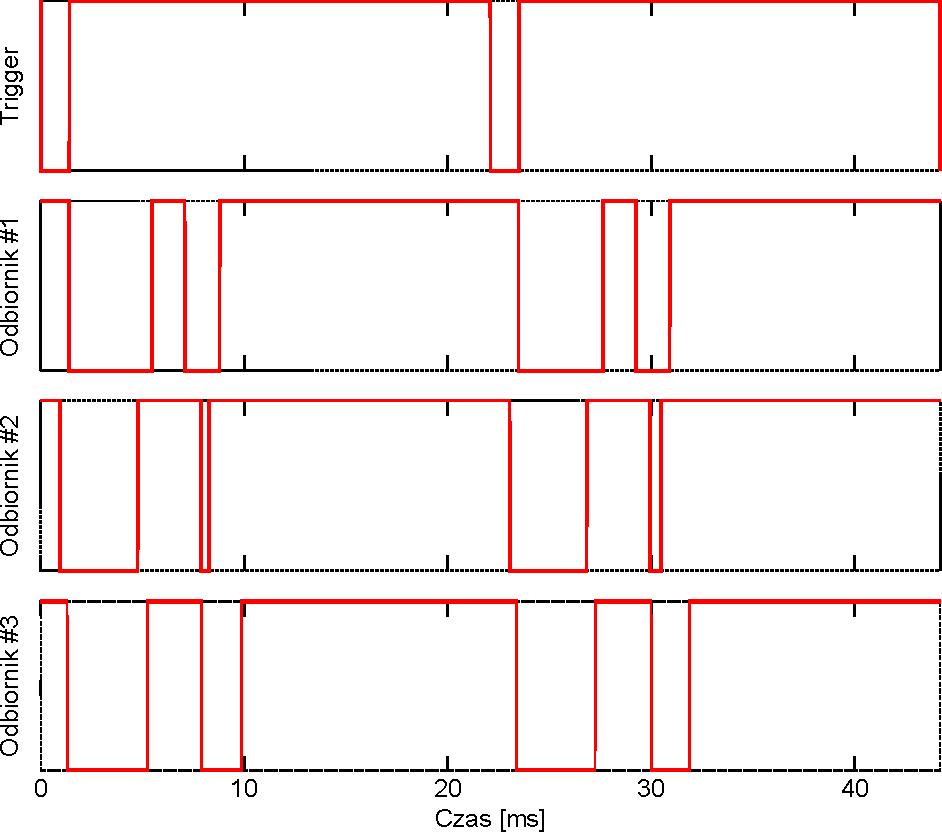
\includegraphics[width=\textwidth]{gfx/odbicia.pdf}
 \caption{Odbicia sygnału dźwiękowego}
 \label{fig:logic_analyzer}
\end{figure}

Porównując długość okresu, w którym nadawany jest sygnał (linia \texttt{Trigger} w stanie niskim) z długością okresu, kiedy odbiornik sygnalizuje odbieranie sygnału (linia odbiornika w stanie niskim), można dostrzec, że nie są one równe. Założyłem, że dźwięk \index{odbicia sygnału}odbił się od pobliskich elementów i dobiegł do odbiornika zanim nastąpił zanik sygnału bezpośredniego.

Na wykresie widać ponadto, że występuje ponowne wygaszenie linii po kilku milisekundach od zakończenia odbierania sygnału. W tym przypadku również zakładałem, że jest to sygnał odbity, który dobiegł do odbiornika.

Dokładniejsze badanie z wykorzystaniem oscyloskopu potwierdzają przypuszczenia. Wyniki tego badania prezentuje rysunek \ref{fig:oscilloscope}\graffito{Sygnał pomiędzy pinem mikrokontrolera, a~punktem testowym jest negowany.}.

\begin{figure}[p]
 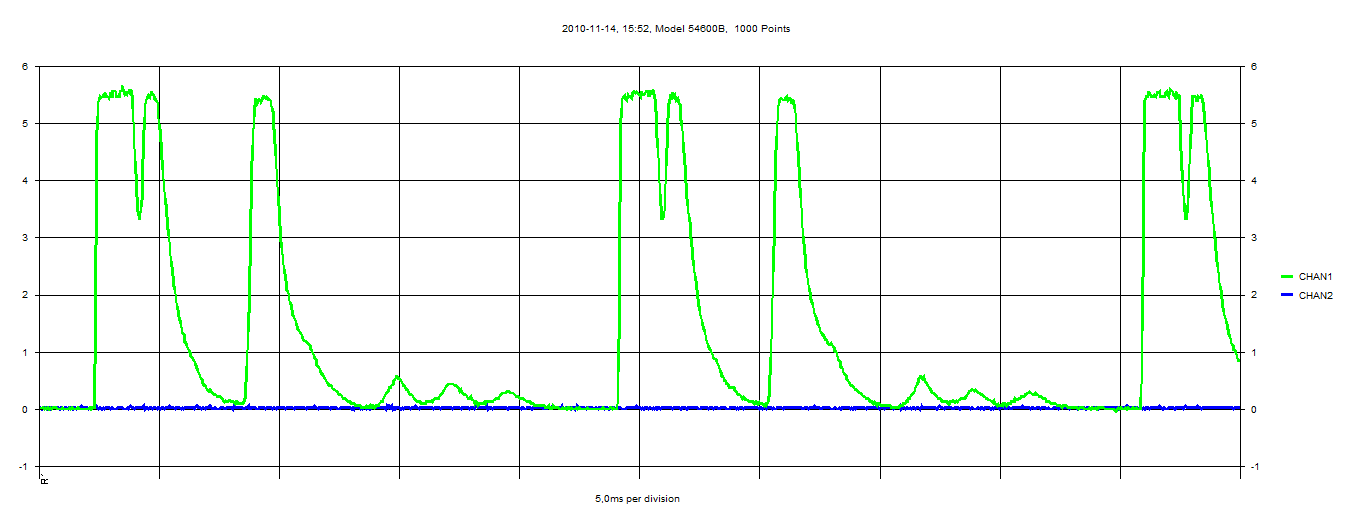
\includegraphics[width=\textwidth]{gfx/oscyloskop_1.png}
 \caption[Oscylogram sygnału w punkcie testowym]{Oscylogram sygnału w jednym z punktów testowych ukazujący odbicia sygnału}
 \label{fig:oscilloscope}
\end{figure}

\begin{figure}[p]
 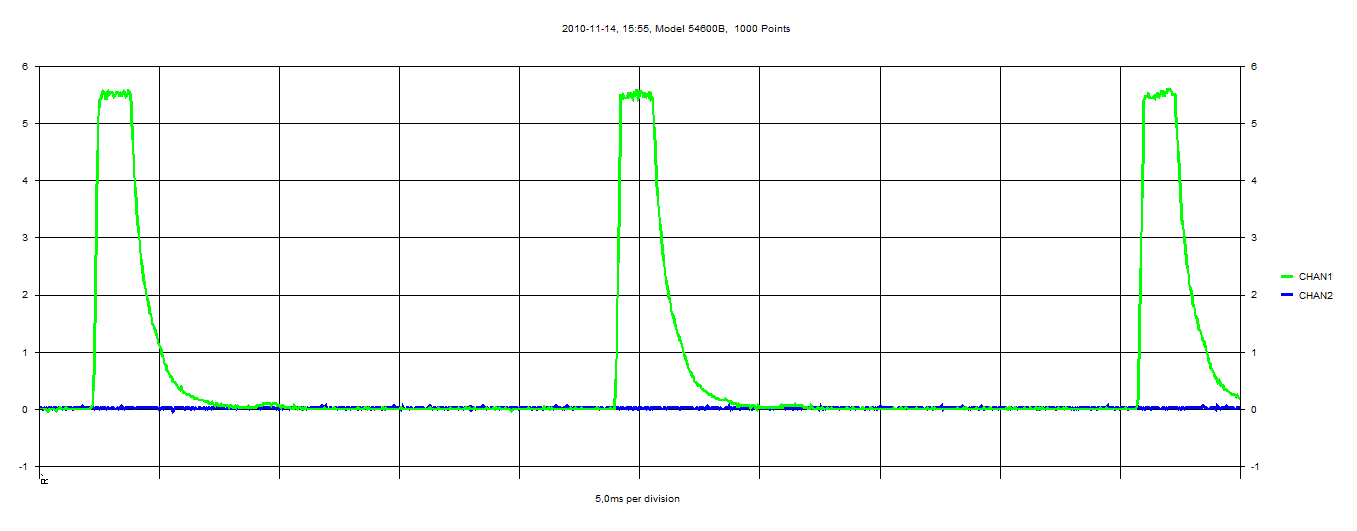
\includegraphics[width=\textwidth]{gfx/oscyloskop_attenuated.png}
 \caption{Oscylogram sygnału z dodatkowym tłumieniem}
 \label{fig:oscilloscope_attenuated}
\end{figure}


Aby uwolnić się od wspomnianej usterki, wprowadziłem do kodu mikrokontrolera wymuszone oczekiwanie, którego zadaniem jest upewnienie się, że wszystkie możliwe odbicia sygnału zaniknęły.

Wprawdzie ,,rozwiązanie'' działa, jednak znacząco spowalnia system \ppauza odstęp pomiędzy próbkami wynosi ponad 20ms.

Inną metodą obejścia tego problemu jest zwiększenie tłumienia sygnału rejestrowanego przez odbiornik. Praktyka pokazuje, że takie działanie faktycznie eliminuje problem, z drugiej jednak strony stanowczo pogarsza sprawność systemu, gdyż wymagane jest wtedy precyzyjniejsze celowanie markerem w odbiorniki. Oscylogram tego badania przedstawia rysunek \ref{fig:oscilloscope_attenuated}.

Z tego też powodu uznałem to za rozwiązanie gorsze, gdyż gracz, który jest docelowym użytkownikiem, w ferworze gry nie może pozwolić sobie na troskanie się sprawnością wykorzystywanego kontrolera.
\newline
\newline
\textsl{Podsumowanie szybkości działania}
Opierając się na wspomnianych powyżej testach widać, że czynnikiem powodującym największe opóźnienia jest dokładnie ten sam, który najtrudniej wyeliminować, czyli odbicia dźwięku. W związku z wprowadzonymi obejściami problemów, wydajność systemu ograniczona jest do najwyżej 25Hz\graffito{Pełen status nadawany jest co minimum 40ms.}.

\paragraph{Porównanie z innymi systemami}
Ze względu na możliwość dostępu do kontrolerów \index{Nintendo!Wiimote}\textsl{Wiimote} oraz \index{Sony!Sixaxis}\textsl{Sixaxis} postanowiłem przeprowadzić porównanie tych urządzeń z moim rozwiązaniem.
\newline

\textsl{Sixaxis}. W celu wyznaczenia prędkości raportowania statusu tego kontrolera wykorzystałem możliwość podłączenia go poprzez port \index{USB}USB oraz obsługę w systemie \index{Linux}Linux w wersji 2.6.35\graffito{Obsługa kontrolera dostępna jest od wersji 2.6.21 z 25.04.2007\citep{Br10}.}. Znając wielkość raportu, która wynosi 50 bajtów \citep{Br10}, wystarczy zbadać, jak prędko dane pojawiają się na urządzeniu przyporządkowanym kontrolerowi. 

Należy najpierw zbadać, do jakiego pliku został przyporządkowany do podłączonego urządzenia \ppauza należy w tym celu sprawdzić log kernela za pomocą polecenia \texttt{dmesg}, a następnie zbadać czas, w jakim odczytana zostanie określona z góry ilość danych. Eksperyment ten prezentuje listing~\ref{lst:sixaxis}.

\begin{listing}
  \lstinputlisting{listings/sixaxis.txt}
  \caption{Badanie prędkości kontrolera Sixaxis}
  \label{lst:sixaxis}
\end{listing}

W celu zbadania prędkości pojawiania się danych wykorzystałem program \texttt{dd} z argumentami:
\begin{description}
 \item[\texttt{if=/dev/hidraw4}] określa plik wejściowy, jest on odczytany z wyjścia programu \texttt{dmesg},
 \item[\texttt{of=/dev/null}] określa plik wyjściowy; przekierowując dane do pliku \texttt{/dev/null} upewniam się, że nie wystąpi ograniczenie prędkości operacją zapisu na dysku,
 \item[\texttt{bs=50}] określa rozmiar bloku danych, dzięki temu ustawiony jest bufor będący w stanie przyjąć cały pakiet danych, przez co unikane jest opóźnienie związane z alokacją pamięci,
 \item[\texttt{count=5000}] informuje program o ilości bloków, jakie mają zostać pobrane; ustaliłem dużą wartość w celu wyeliminowania opóźnień, jakie mogłyby wyniknąć w związku z inicjacją i zakończeniem transmisji.
\end{description}

Jak widać, w ciągu prawie dokładnie 50s przetransmitowanych zostało dokładnie 250000 bajtów. Wynika stąd, że prędkość raportowania wynosi
\begin{equation}
 \frac{250000\textrm{b}}{50\textrm{s}} : 50\frac{\textrm{b}}{\textrm{raport}} = 100\textrm{Hz}
\end{equation}

Analizując strukturę raportu, łatwo rozpoznać przyporządkowanie danych do przycisków i policzyć ilość przycisków ,,analogowych''\graffito{Przyciskami analogowymi zwykło nazywać się przyciski, które raportują jak bardzo są naciśnięte.}.
\newline

\index{Nintendo!Wiimote}\textsl{Wiimote}. W celu zbadania tego kontrolera wykorzystałem otwartoźródłową bibliotekę \texttt{CWiid}\citep{CWiid}. Zmodyfikowałem źródło jednego z programów, aby raportował czas przyjścia raportu, a następnie w oparciu o informacje o rozmiarach raportów (\citep{Wiibrew}) wybrałem raport, którego rozmiar wynosi dokładnie 18 bajtów, po czym obliczyłem ile raportów przyszło w danym okresie czasu.

Wyniki tego testu pokazuje listing~\ref{lst:wiimote}.

\begin{listing}
  \lstinputlisting{listings/wiimote.txt}
  \caption{Badanie prędkości kontrolera Wiimote}
  \label{lst:wiimote}
\end{listing}

Do pliku \texttt{log} zapisane zostały czasy w formacie \textit{sekundy.nanosekundy}\graffito{W systemach Linux czas reprezentowany jest jako ilość sekund od 1970-01-01T00:00:00Z (ISO 8601).}. W każdej linii pliku zapisana jest dokładnie jedna próbka, dlatego też ilość pobranych próbek wynosi 2500, co pokazuje program \texttt{wc} z argumentem \texttt{-l}. Różnicę pomiędzy rozpoczęciem, a zakończeniem rejestrowania danych prezentuje wynik działania programu \texttt{bc}. Wynika stąd, że prędkość raportowania wynosi
\begin{equation}
 \frac{2500}{25,45\textrm{s}} \approx 100\textrm{Hz}
\end{equation}

Porównanie tych i pozostałych parametrów kontrolerów prezentuje tabela \ref{tab:comparison}.


% http://texblog.net/latex-archive/layout/centering-figure-table/
\begin{table}[b]
  \myfloatalign
\noindent\makebox[\textwidth]{%
\index{Bluetooth} \index{USB} \index{RS232} \index{akcelerometr} \index{żyroskop} \index{Sony!Sixaxis} \index{Nintendo!Wiimote}
\begin{tabularx}{1.5\textwidth}{X|XXX} \toprule
    & \emph{Sixaxis} & \emph{Wiimote} & \emph{Nietoperz} \\ \hline
    Ilość przycisków & 17 & 11 & 0 \\
    Ilość przycisków ,,analogowych'' & 12 (nie licząc gałek) & 0 & 0 \\
    Komunikacja & Bluetooth, USB & Bluetooth & RS232 \\
    Prędkość raportowania & 100Hz & do 100Hz & poniżej 25Hz \\
    Wielkość raportu statusu & 50 bajtów & do 18 bajtów & 16 bajtów \\
    Możliwość dołączania rozszerzeń & \texttimes & \checkmark & \texttimes \\
    Detekcja ruchów & akcelerometr (3D), żyroskop (1D) & akcelerometr (3D) & ultradźwięki \\
    Dodatkowe funkcjonalności & zdalne uruchamianie konsoli, 4 diody, 2 gałki analogowe & zdalne uruchamianie konsoli, głośnik, kamera IR, 4 diody & 8 diod
  \end{tabularx}}
  \caption{Zestawienie funkcjonalności kontrolerów gier}
  \label{tab:comparison}
\end{table}
\myChapter{Podsumowanie}\label{ch:conclusion}
%************************************************

Udało mi się zrealizować założenia, które przewidywała moja praca inżynierska.

Niestety nie udało się zawrzeć dodatkowych funkcjonalności, które znacznie zwiększyłyby możliwości systemu i sprawiłyby, że stałby się znacznie bardziej ciekawą propozycją.

Chociaż konstrukcja sprzętu nie należy do zakresu tej pracy, to możliwość udziału w projektowaniu całego systemu stanowiła przyjemną odskocznię od programów tworzonych na zajęcia na uczelni. Praca z systemem dała dużą satysfakcję ze względu na działanie z realnym urządzeniem, a nie tylko i wyłącznie algorytmem zapisanym w pamięci komputera.

%Uważam, że moja praca jest interesująca również dlatego, że działa ona po części także poza komputerem, co powoduje,

Podsumowując pracę związaną z projektem, zamieszczam listę wad i zalet systemu.

Główne wady to:
\begin{aenumerate}
 \item niestabilność \ppauza próbki wykazują relatywnie duże zmiany pomimo stabilności markerów,
 \item zawodność \ppauza aby system działał sprawnie, wymagane jest celowanie markerem w stronę odbiorników, co uniemożliwia sprawne wykorzystywanie systemu bez obawy o zgubienie pozycji,
 \item mała szybkość \ppauza firmy produkujące myszki i klawiatury dla graczy prześcigują się w technologiach możliwie najszybszych czasów reakcji, natomiast \textsl{Nietoperz} osiąga szybkość zaledwie 25Hz; nawet jeśli byłaby możliwość przyspieszenia, to i tak pozostawałaby ta wartość daleko w tyle za 100Hz, którą mogą poszczycić się prawdziwe kontrolery,
 \item możliwość korzystania tylko przez jedną osobę \ppauza eliminuje możliwość gry zespołowej,
 \item konieczność kalibracji \ppauza może zniechęcać do korzystania z systemu, ponadto przypadkowe przesunięcia \textsl{Nietoperza} względem użytkownika mogą być odczytywane jako niepożądany ruch.
\end{aenumerate}

Do zalet systemu można natomiast zaliczyć:
\begin{aenumerate}
 \item niskie koszty \ppauza odtworzenie całości systemu jest na każdą kieszeń,
 \item innowacyjność \ppauza wykorzystałem metodę, jaka nie była zastosowana do tej pory w konsolach do gier,
 \item prostota \ppauza zasada działania \textsl{Nietoperza} opiera się o podstawową geometrię, łatwo więc zrozumieć metodę jego działania.
\end{aenumerate}

%Przeprowadzone porównanie, a także korzystanie z systemu, pokazuje, że nie jest on wystarczająco wydajny, a także dostarcza niedostatecznie stabilnych wyników, aby można było go stosować jako system manipulacji.

Z przykrością muszę stwierdzić, że wady systemu przeważają jego zalety, zatem uznaję go za niezdatny jako interfejs człowiek-komputer, a w szczególności jako kontroler do gier. \textsl{Nietoperz} pozostanie jednak interesującym eksperymentem, który być może znajdzie jeszcze jakieś niszowe zastosowanie.
%\include{multiToC}
% ********************************************************************
% Backmatter
%*******************************************************
%\appendix
%\cleardoublepage\myPart{Appendix}
%%********************************************************************
% Appendix
%*******************************************************
\myChapter{Appendix Test}
Lorem ipsum at nusquam appellantur his, ut eos erant homero
concludaturque. Albucius appellantur deterruisset id eam, vivendum
partiendo dissentiet ei ius. Vis melius facilisis ea, sea id convenire
referrentur, takimata adolescens ex duo. Ei harum argumentum per. Eam
vidit exerci appetere ad, ut vel zzril intellegam interpretaris.

Errem omnium ea per, pro congue populo ornatus cu, ex qui dicant
nemore melius. No pri diam iriure euismod. Graecis eleifend
appellantur quo id. Id corpora inimicus nam, facer nonummy ne pro,
kasd repudiandae ei mei. Mea menandri mediocrem dissentiet cu, ex
nominati imperdiet nec, sea odio duis vocent ei. Tempor everti
appareat cu ius, ridens audiam an qui, aliquid admodum conceptam ne
qui. Vis ea melius nostrum, mel alienum euripidis eu.

\section{Appendix Section Test}
Ei choro aeterno antiopam mea, labitur bonorum pri no. His no decore
nemore graecis. In eos meis nominavi, liber soluta vim cu. Sea commune
suavitate interpretaris eu, vix eu libris efficiantur.

\graffito{More dummy text.}
Nulla fastidii ea ius, exerci suscipit instructior te nam, in ullum
postulant quo. Congue quaestio philosophia his at, sea odio autem
vulputate ex. Cu usu mucius iisque voluptua. Sit maiorum propriae at,
ea cum primis intellegat. Hinc cotidieque reprehendunt eu nec. Autem
timeam deleniti usu id, in nec nibh altera.

\section{Another Appendix Section Test}
Equidem detraxit cu nam, vix eu delenit periculis. Eos ut vero
constituto, no vidit propriae complectitur sea. Diceret nonummy in
has, no qui eligendi recteque consetetur. Mel eu dictas suscipiantur,
et sed placerat oporteat. At ipsum electram mei, ad aeque atomorum
mea.

\begin{table}
    \myfloatalign
  \begin{tabularx}{\textwidth}{Xll} \toprule
    \tableheadline{labitur bonorum pri no} & \tableheadline{que vista}
    & \tableheadline{human} \\ \midrule
    fastidii ea ius & germano &  demonstratea \\
    suscipit instructior & titulo & personas \\
    %postulant quo & westeuropee & sanctificatec \\
    \midrule
    quaestio philosophia & facto & demonstrated \\
    %autem vulputate ex & parola & romanic \\
    %usu mucius iisque & studio & sanctificatef \\
    \bottomrule
  \end{tabularx}
  \caption[Autem usu id]{Autem usu id.}
  \label{tab:moreexample}
\end{table}

Ei solet nemore consectetuer nam. Ad eam porro impetus, te choro omnes
evertitur mel. Molestie conclusionemque vel at, no qui omittam
expetenda efficiendi. Eu quo nobis offendit, verterem scriptorem ne
vix.

%********************************************************************
% Other Stuff in the Back
%*******************************************************
\cleardoublepage%********************************************************************
% Bibliography
%*******************************************************
% work-around to have small caps also here in the headline
\manualmark
\markboth{\spacedlowsmallcaps{\bibname}}{\spacedlowsmallcaps{\bibname}} % work-around to have small caps also
%\phantomsection 
\refstepcounter{dummy}
\addtocontents{toc}{\protect\vspace{\beforebibskip}} % to have the bib a bit from the rest in the toc
\addcontentsline{toc}{chapter}{\tocEntry{\bibname}}
\bibliographystyle{janisozaurowy}
% http://win.ua.ac.be/~nschloe/content/bibtex-how-cite-website
\label{app:bibliography} 
\bibliography{Bibliography}
\cleardoublepage\pagestyle{empty}

\hfill

\vfill


\pdfbookmark[0]{Colophon}{colophon}
\section*{Colophon}
Colophon, as included with the used style.

This thesis was typeset with \LaTeXe\ using Hermann Zapf's
\emph{Palatino}
and \emph{Euler} type faces (Type~1 PostScript fonts \emph{URW
Palladio L}
and \emph{FPL} were used). The listings are typeset in \emph{Bera
Mono}, originally developed by Bitstream, Inc. as ``Bitstream Vera''.
(Type~1 PostScript fonts were made available by Malte Rosenau and
Ulrich Dirr.)

The typographic style was inspired by Bringhurst's genius as
presented in \emph{The Elements of Typographic Style} 
\citep{bringhurst2002}. It is available for \LaTeX\ via \textsmaller{CTAN} as 
``\href{http://www.ctan.org/tex-archive/macros/latex/contrib/classicthesis/}%
{\texttt{classicthesis}}''.

\paragraph{note:} The custom size of the textblock was calculated
using the directions given by Mr. Bringhurst (pages 26--29 and
175/176). 10~pt Palatino needs  133.21~pt for the string
``abcdefghijklmnopqrstuvwxyz''. This yields a good line length between
24--26~pc (288--312~pt). Using a ``\emph{double square textblock}''
with a 1:2 ratio this results in a textblock of 312:624~pt (which
includes the headline in this design). A good alternative would be the
``\emph{golden section textblock}'' with a ratio of 1:1.62, here
312:505.44~pt. For comparison, \texttt{DIV9} of the \texttt{typearea}
package results in a line length of 389~pt (32.4~pc), which is by far
too long. However, this information will only be of interest for
hardcore pseudo-typographers like me.%

To make your own calculations, use the following commands and look up
the corresponding lengths in the book:
\begin{verbatim}
    \settowidth{\abcd}{abcdefghijklmnopqrstuvwxyz}
    \the\abcd\ % prints the value of the length
\end{verbatim}
Please see the file \texttt{classicthesis.sty} for some precalculated 
values for Palatino and Minion.

%    \settowidth{\abcd}{abcdefghijklmnopqrstuvwxyz}
%    \the\abcd\ % prints the value of the length


\bigskip

\noindent\finalVersionString




\cleardoublepage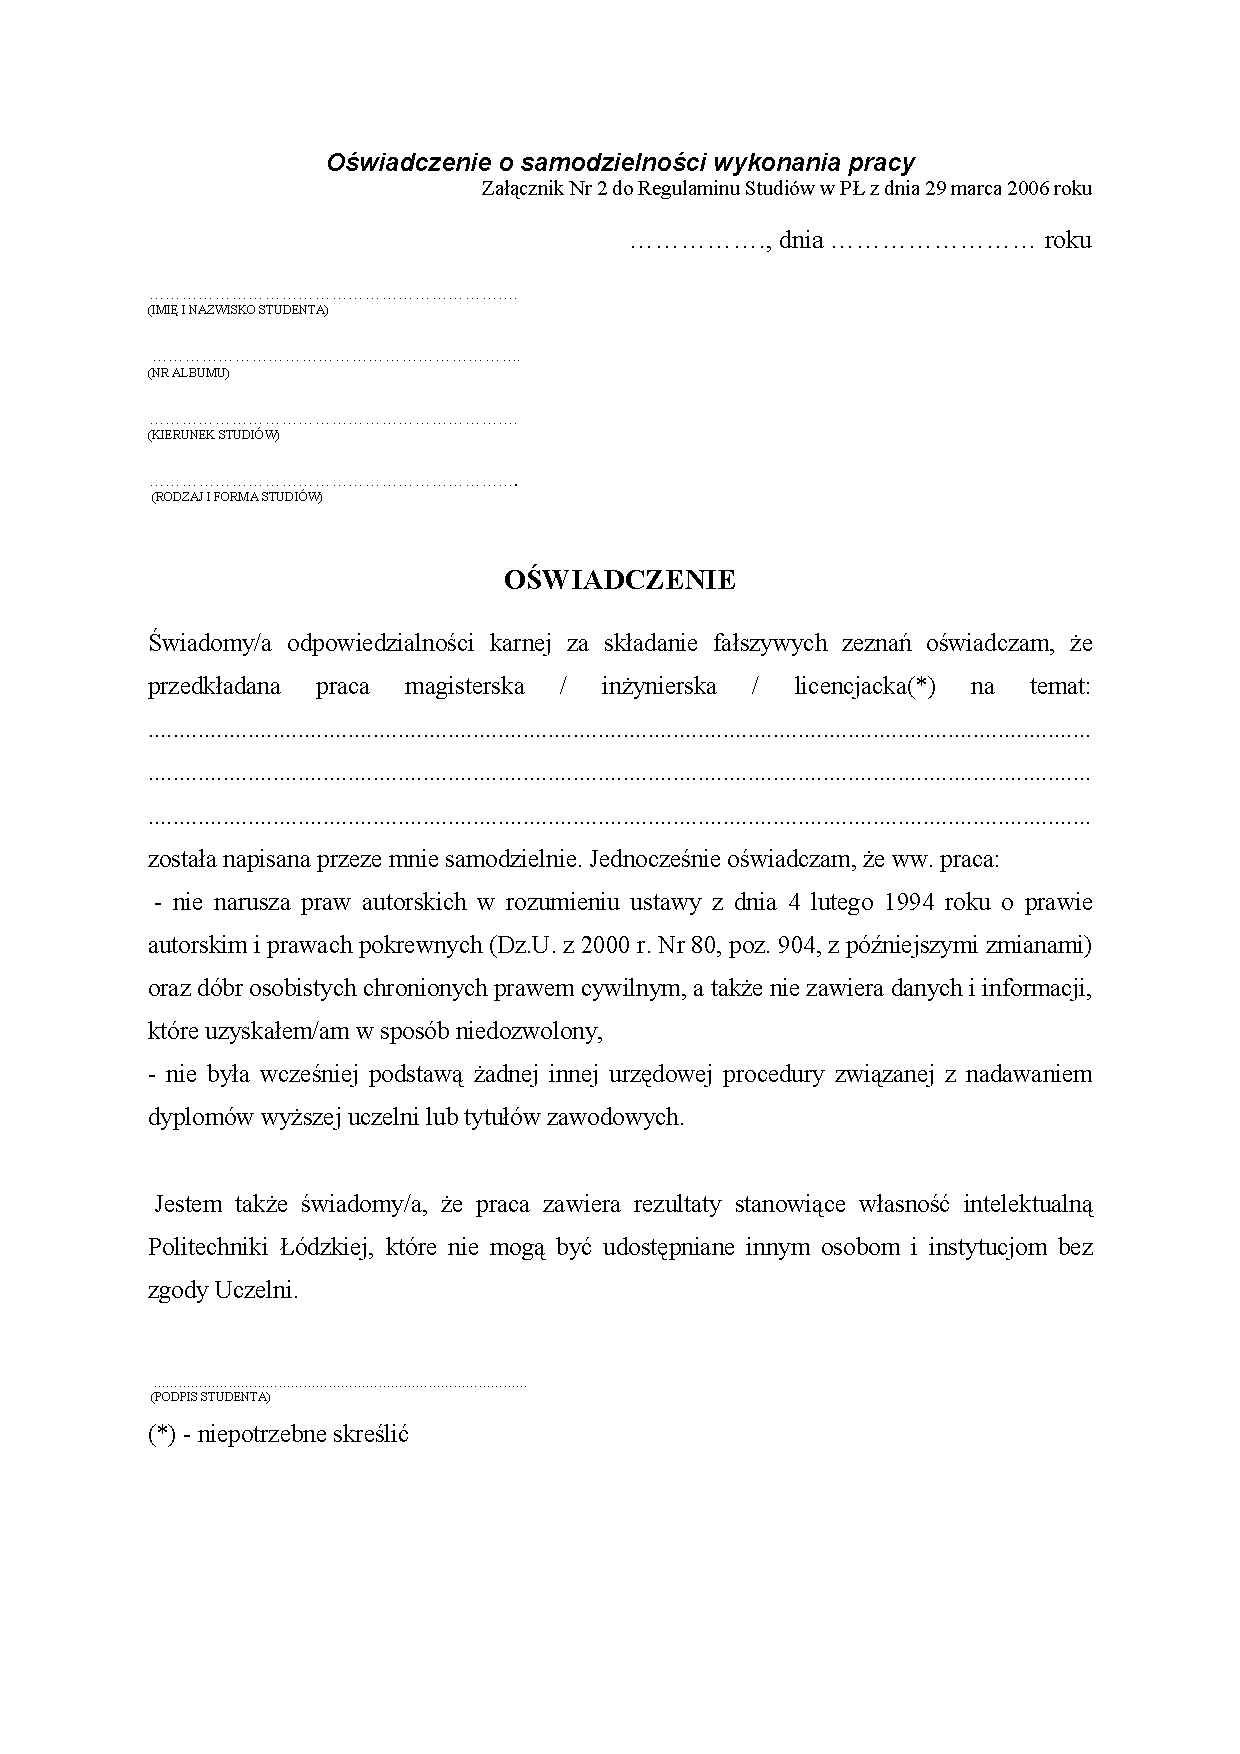
\includepdf[pagecommand={\thispagestyle{empty}}]{FrontBackmatter/declaration.pdf}
% ********************************************************************
% Game Over: Restart, Restore or Quit?
%*******************************************************
\end{document}
% ********************************************************************
